%http://www.daniel-brettschneider.de/allgemein/latex-vorlage-fur-hausarbeiten-oder-abschlussarbeiten

\documentclass[12pt,a4paper,bibliography=totocnumbered,listof=totocnumbered]{scrartcl}
\usepackage[ngerman]{babel}
\usepackage[utf8]{inputenc}
\usepackage{amsmath}
\usepackage{amsfonts}
\usepackage{amssymb}
\usepackage{graphicx}
\usepackage{fancyhdr}
\usepackage{tabularx}
\usepackage{geometry}
\usepackage{setspace}
\usepackage[right]{eurosym}
\usepackage[printonlyused]{acronym}
\usepackage{subfig}
\usepackage{floatflt}
\usepackage{float}
\usepackage{placeins}
\usepackage[usenames,dvipsnames]{color}
\usepackage{colortbl}
\usepackage{paralist}
\usepackage{array}
\usepackage{titlesec}
\usepackage{parskip}
\usepackage{booktabs}
\usepackage[right]{eurosym}
\usepackage{picins}
\usepackage[subfigure,titles]{tocloft}
\usepackage[pdfpagelabels=true]{hyperref}
\usepackage{listings}
\usepackage{colortbl}
\lstset{language=C}  


%für Listings
\usepackage{listings}
\lstset{basicstyle=\footnotesize, captionpos=b, breaklines=true, showstringspaces=false, tabsize=2, frame=lines, numbers=left, numberstyle=\tiny, xleftmargin=2em, framexleftmargin=2em}
\makeatletter
\def\l@lstlisting#1#2{\@dottedtocline{1}{0em}{1em}{\hspace{1,5em} Lst. #1}{#2}}
\makeatother




\newcommand{\includecode}[1]{\lstinputlisting[caption=#1]{#1}}

%Seitenränder
\geometry{a4paper, top=27mm, left=30mm, right=20mm, bottom=35mm, headsep=10mm, footskip=12mm}

%Links und PDF-Einstellungen
\hypersetup{unicode=false, pdftoolbar=true, pdfmenubar=true, pdffitwindow=false, pdfstartview={FitH},
	pdftitle={Projektdokumentation},
	pdfauthor={Daniel Kreck, Leonard Schmischke, Thomas Iffland, Ewald Bayer, Sebastian Westbrock},
	pdfsubject={Projektdokumentation Ada-Instant-Messenger},
	pdfcreator={\LaTeX\ with package \flqq hyperref\frqq},
	pdfproducer={pdfTeX \the\pdftexversion.\pdftexrevision},
	pdfkeywords={Dokumentation, Projekt, Ada, Chat},
	pdfnewwindow=true,
	colorlinks=true,linkcolor=black,citecolor=black,filecolor=magenta,urlcolor=black}
\pdfinfo{/CreationDate (D:20110620133321)}

\begin{document}

\titlespacing{\section}{0pt}{12pt plus 4pt minus 2pt}{-6pt plus 2pt minus 2pt}

% Kopf- und Fusszeile
\renewcommand{\sectionmark}[1]{\markright{#1}}
\renewcommand{\leftmark}{\rightmark}
\pagestyle{fancy}
\lhead{}
\chead{}
\rhead{\thesection\space\contentsname}
\lfoot{Projektdokumentation}
\cfoot{}
\rfoot{ Seite \thepage}
\renewcommand{\headrulewidth}{0.4pt}
\renewcommand{\footrulewidth}{0.4pt}

% Vorspann
\renewcommand{\thesection}{\Roman{section}}
\renewcommand{\theHsection}{\Roman{section}}
\pagenumbering{arabic}

% ----------------------------------------------------------------------------------------------------------
% Titelseite
% ----------------------------------------------------------------------------------------------------------

\thispagestyle{empty}
\begin{center}
	
\includegraphics[width=5cm]{img/thm2.png}\\
	\vspace*{2cm}
	\Large
	\textbf{Fachbereich}\\
	\textbf{Mathematik, Naturwissenschaften und Informatik }\\
	\vspace*{2cm}
	\Huge
	\textbf{Projektdokumentation Instant-Messaging-Dienst}\\
	\vspace*{1cm}
	\large
	\textbf{Entwicklung sicherer, hardwarenaher Anwendungen}\\
	\normalsize
	\vspace*{0.5cm}
	Wintersemester 15/16\\
	\vspace*{2cm}
	\textbf{Stand: 30.04.2016}
	
	\normalsize
	\vfill
	\begin{tabular}{ l l }
		\textbf{Projektleiter:}  & \textbf{Projektteam:}\\
		Leonard Schmischke & Daniel Kreck\\
		&  Ewald Bayer\\
		\textbf{Kursleitung:} & Sebastian Westbrock\\
		Florian von Zabiensky & Thomas Iffland\\
	\end{tabular}	
\end{center}

\pagebreak

% ----------------------------------------------------------------------------------------------------------
% Verzeichnisse
% ----------------------------------------------------------------------------------------------------------
% TODO Typ vor Nummer
\renewcommand{\cfttabpresnum}{Tab. }
\renewcommand{\cftfigpresnum}{Abb. }
\settowidth{\cfttabnumwidth}{Abb. 10\quad}
\settowidth{\cftfignumwidth}{Abb. 10\quad}

\titlespacing{\section}{0pt}{12pt plus 4pt minus 2pt}{2pt plus 2pt minus 2pt}
\singlespacing
\rhead{INHALTSVERZEICHNIS}
\renewcommand{\contentsname}{Inhaltsverzeichnis}
\tableofcontents
\pagebreak


% ----------------------------------------------------------------------------------------------------------
% Inhalt
% ----------------------------------------------------------------------------------------------------------
% Abstände Überschrift
\titlespacing{\section}{0pt}{12pt plus 4pt minus 2pt}{-6pt plus 2pt minus 2pt}
\titlespacing{\subsection}{0pt}{12pt plus 4pt minus 2pt}{-6pt plus 2pt minus 2pt}
\titlespacing{\subsubsection}{0pt}{12pt plus 4pt minus 2pt}{-6pt plus 2pt minus 2pt}

% Kopfzeile
\renewcommand{\sectionmark}[1]{\markright{#1}}
\renewcommand{\subsectionmark}[1]{}
\renewcommand{\subsubsectionmark}[1]{}
\lhead{Kapitel \thesection}
\rhead{\rightmark}

\onehalfspacing
\renewcommand{\thesection}{\arabic{section}}
\renewcommand{\theHsection}{\arabic{section}}
\setcounter{section}{0}

\section{Projektidee}
Lastenheft etc.

% ----------------------------------------------------------------------------------------------------------
% Architektur
% ----------------------------------------------------------------------------------------------------------
\section{Architektur}
bla bla

\subsection{Kommunikationsprotokoll}
Eine Nachricht besteht aus vier Komponenten:

\vspace{1em}
\begin{minipage}{\linewidth}
	\centering
	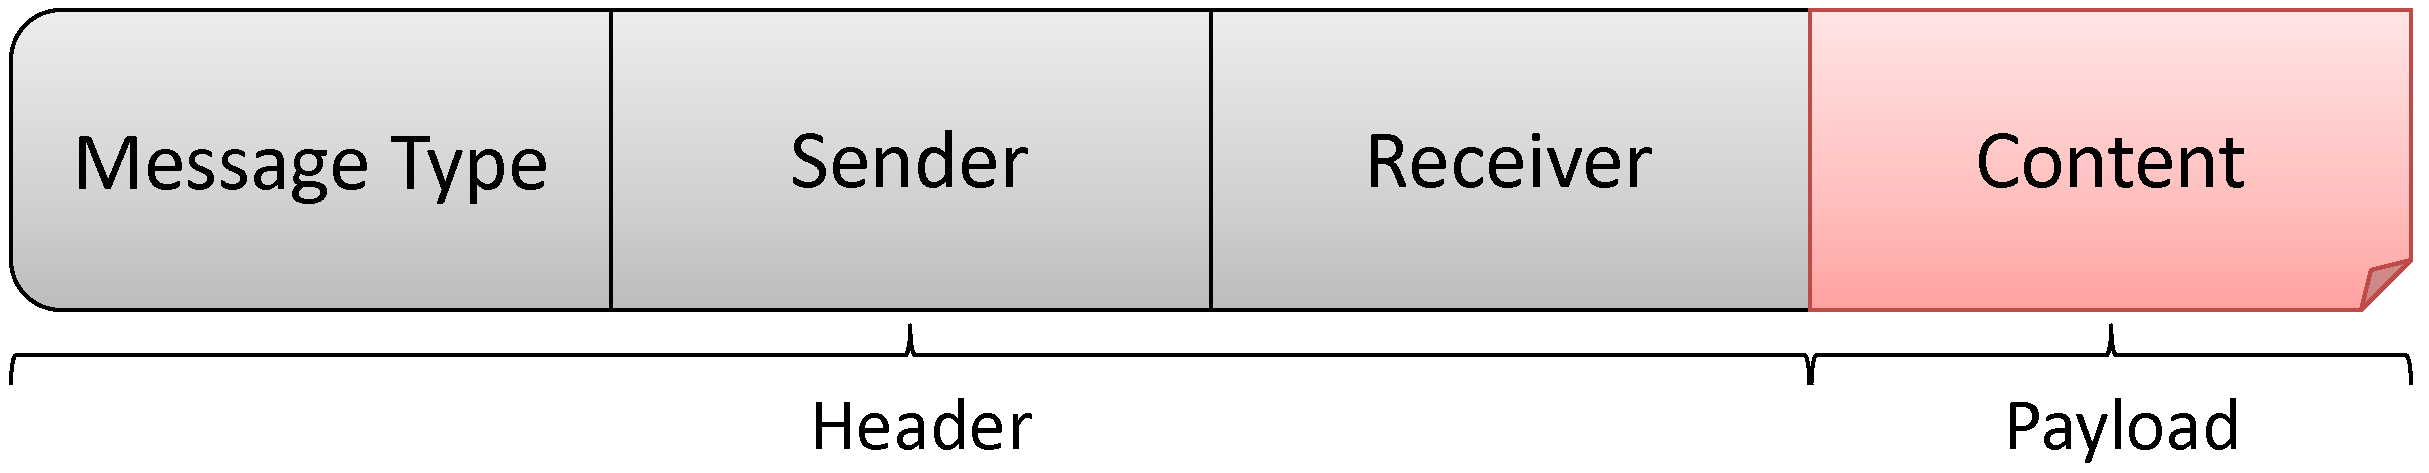
\includegraphics[width=0.7\linewidth]{img/Nachrichtenstruktur.png}
	\captionof{figure}[Nachrichtenstruktur]{Struktur einer Nachricht}
	\label{fig:Nachrichtenstruktur}
\end{minipage}
\vspace{0.5em}

Die einzelnen Teile einer Nachricht werden durch ein definiertes Trennzeichen separiert. Hierbei handelt es sich um ein nicht druckbares Zeichen um den Zeichenraum der Nutzer beim Chatten nicht unnötig einzuschränken.

Während Bestandteile des Headers nicht mehr weiter unterteilbar sind, wird der Inhalt je nach Nachrichtentyp noch feiner strukturiert, indem in ihm das gleiche Trennzeichen wiederholt zur Anwendung kommt.

Der Nachrichtentyp wird durch die Definition eines Aufzählungstypen von 13 zu unterscheidenden Werten realisiert. Das Absender-Feld hält den Namen des Benutzers als Zeichenkette fest, wohingegen das Empfänger-Feld den Chatraum als positive Ganzahl kodiert. Dies hat den Grund, dass zur Kommunikation immer ein Chatraum erforderlich ist. Alle Nachrichten werden zunächst als Broadcast gehandhabt, allerdings kann durch einen Chatraum von zwei Nutzern Unicast-Kommunikation verwirklicht werden.

Bei diesem Vorgehen nimmt der Chatraum mit der Nummer \textit{0} eine besondere Rolle ein, da er statisch erzeugt und immer da ist. Er ist die Anlaufstelle für eingehende Verbindungsanfragen, da erst im Folgenden Schritt dem anfragenden Client dynamisch ein einzelner Chatraum zur Kommunikation mit dem Server zugewiesen werden kann. Nach dem Verbindungsaufbau verfügt demnach jeder Client über einen eigenen Server-Chatraum und ggf. wenn er die Kommunikation mit anderen Clients sucht, über jeweils einen Chatraum für jeden Kommunikationspartner. Diese werden zunächst als Einzelchats zwischen zwei Nutzern erzeugt, können aber durch Benutzerinteraktion um beliebig viele Teilnehmer erweitert werden, wodurch Gruppenkommunikation möglich ist.

\subsubsection{Registrierung}
Zu Anfang wird dem Benutzer, bevor er anderweitige Funktionalität des Programmes nutzen kann, eine Registrierung mit freiwählbarem Benutzernamen und Passwort abverlangt. 

Hierzu schreibt das Protokoll folgendes Verhalten vor: 
Der Client sendet eine Registrierungsanfrage an den Server. Diese ist vom Nachrichtentyp \textit{register} und trägt im Absender-Feld den gewünschten Benutzernamen. Als Receiver wird der Standard-Chatraum des Servers angegeben. Der Inhalt der Nachricht ist das verschlüsselt zu übertragende Passwort des Benutzers.

\vspace{1em}
\begin{minipage}{\linewidth}
	\centering
	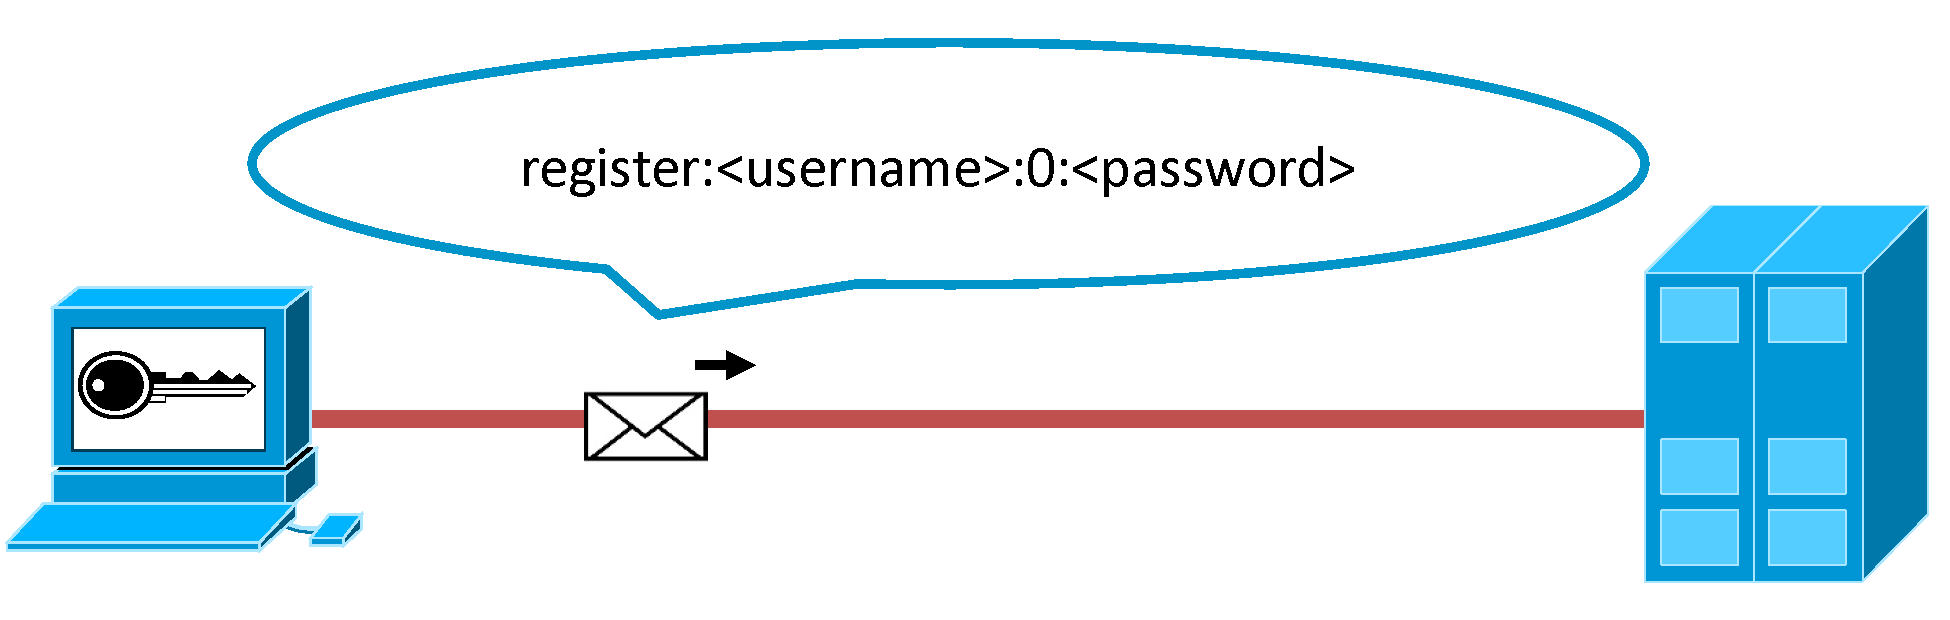
\includegraphics[width=0.7\linewidth]{img/register1.png}
	\label{fig:Registrierung1}
\end{minipage}
\vspace{0.5em}

Wenn der Server die Nachricht empfängt quittiert er den Erfolgsfall, indem ebenfalls eine  \textit{register}-Nachricht, mit dem Inhalt \glqq ok\grqq{} zurückgeschickt wird. Sollte der Benutzername bereits verwendet werden, wird eine \textit{refused}-Nachricht mit Inhalt \glqq registration failed, name in use\grqq{} versendet.

\vspace{1em}
\begin{minipage}{\linewidth}
	\centering
	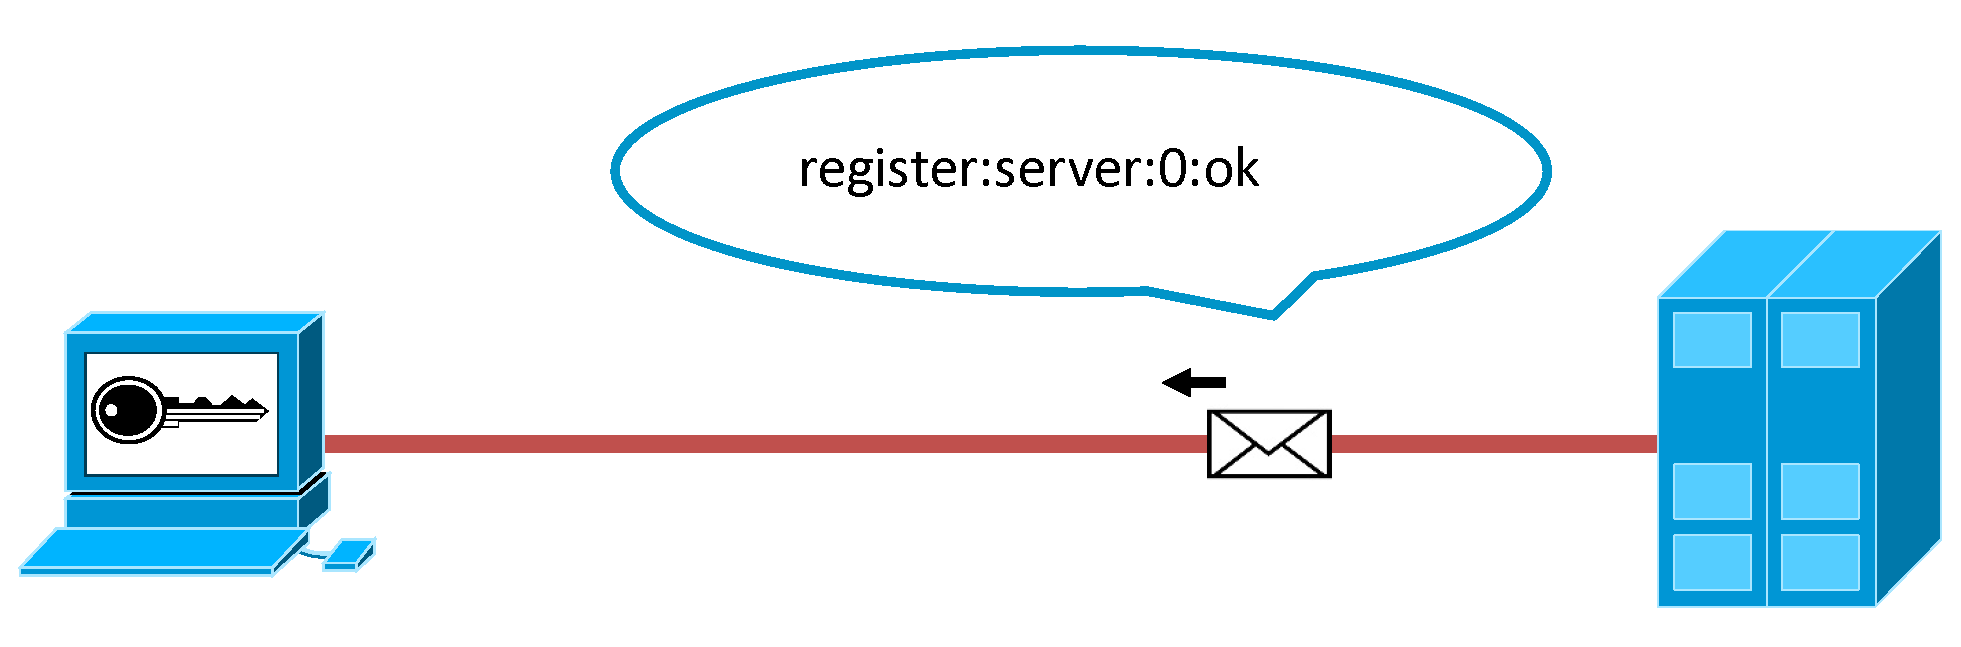
\includegraphics[width=0.7\linewidth]{img/register2.png}
	\label{fig:Registrierung2}
\end{minipage}
\vspace{0.5em}

\subsubsection{Verbindungsaufbau}

\subsubsection{Kontaktanfrage}

\subsubsection{Kommunikation}

\subsubsection{Verbindungsabbau}

\subsection{Klassendiagramm}

% ----------------------------------------------------------------------------------------------------------
% Vorgehen
% ----------------------------------------------------------------------------------------------------------
\section{Vorgehen}
Usecases definiert

Skizzen für GUIs erstellt

aufteilen des Klassendiagramms auf die Leute, wöchentliche Treffen


\subsection{dies und das}
bla bla

% ----------------------------------------------------------------------------------------------------------
% Probleme
% ----------------------------------------------------------------------------------------------------------
\section{Probleme}
Arbeiten mit GTK

fehlende ausführliche Dokumentation für GTK und ADA (und Beispiele im Internet)

Zirkuläre Abhängigkeiten

Merkwürdigkeiten in ADA (Endlosschleife durch If-Abfrage)

\subsection{dies und das}
bla bla

\pagebreak


% ----------------------------------------------------------------------------------------------------------
% Praktische Praktikumsaufgaben
% Code und so weit vorhanden Vorüberlegungen, Entwurfsunterlagen, Algorithmen, Kommentare, Schaltpläne, Messergebnisse, Diagramme usw. zu den Aufgaben ----------------------------------------------------------------------------------------------------------
\section{Praktische Aufgabenstellungen}

In diesem Abschnitt werden die fünf Kernaufgaben aus dem Mikroprozessortechnik-Praktikum durch Darstellung der Vorüberlegungen, Auflistung von Diagrammen und des Quellcodes ausführlich beschrieben.

\subsection{Endfassung Lauflicht}
Diese Aufgabe verfolgt das Ziel, dass die Studierenden Erste Schritte mit den im Praktikum verwendeten Arbeitsmitteln machen können.
Hierzu kommt der Mikrocontroller MSP430 von Texas Instruments, ein Education Board des FTZ Leipzig, sowie die IAR Embedded Workbench IDE zum Einsatz.

Die Aufgabe besteht darin, ein C-Programm zu schreiben, dass die acht auf dem Praktikumsboard aufgebrachten Leuchtdioden endlos von rechts nach links und wieder zurück aufblinken lässt, sodass ein Lauflicht entsteht.

Zu beachten ist, dass die Logik invertiert ist. Das heißt ein Low-Pegel auf den LED-Ports (festgelegt in P1OUT) führt zum Leuchten der LED und ein High-Pegel zu deren erlöschen.

Bevor die LEDs angesprochen werden können, müssen die entsprechenden Leitungen als Ausgabeport geschaltet werden.

\vspace{1em}
\lstinputlisting[caption={Port-Direction konfigurieren, alle Pins sind Ausgänge}]{src/Lauflicht/P1DIR.c}

Damit das menschliche Auge Zeit hat, das Leuchten einer LED wahrzunehmen, wird durch eine Warteschleife am Ende jedes Schaltvorgangs eine Verzögerung umgesetzt.

\vspace{1em}
\lstinputlisting[caption=Implementierung der Warteschleife]{src/Lauflicht/Warteschleife.c}

Anschließend wird das an P1OUT anliegende Bitmuster durch eine Shift-Operation nach links beziehungsweise rechts geschoben, um das Lauflicht zu erzeugen.

\vspace{1em}
\lstinputlisting[caption=Wandern der LEDs]{src/Lauflicht/Schleife.c}

Das vollständige Programm kann Anhang \ref{sec:Lauflicht} entnommen werden.

\pagebreak

\subsection{Endfassung Taschenrechner}
\label{Taschenrechner}
Es soll ein Taschenrechner entwickelt werden, der folgende Grundoperationen ausführen kann:
\begin{itemize}
	\item aktueller Zahlenwert wird um 1 erhöht
	\item aktueller Zahlenwert wird um 1 erniedrigt
	\item aktueller Zahlenwert wird verdoppelt
	\item aktueller Zahlenwert wird halbiert (Rest entfällt)
\end{itemize}
Die Bedienung des Taschenrechners soll über die Tasten des Education Boards erfolgen. Das Betätigen derer löst ein Interrupt aus, welches vom MSP430 behandelt werden soll. Der aktuellen Zahlenwert wird auf dem Display und durch die LEDs dargestellt.

Zuerst werden die LEDs wie auch schon in der letzten Aufgabe konfiguriert, indem alle Portpins auf Ausgabe geschaltet werden.

Anschließend werden jeweils die Bits 0, 1, 2 und 5 im P2IE- und P2IES-Register gesetzt, um für die jeweiligen Pins Interrupts bei fallender Flanke freizuschalten. Die genannten Bits entsprechen den Tasten des Education Boards.

\vspace{1em}
\lstinputlisting[caption=Konfiguration der Interrupt-Register des Port 2]{src/TR/P2Interrupts.c}

Nun können also durch das Betätigen der Tasten Interrupts ausgelöst werden, die in der Interrupt Service Routine bearbeitet werden müssen.

Durch Auswertung des P2IFG-Registers kann festgestellt werden, welche Taste den Interrupt ausgelöst hat. Hierzu werden Makros definiert, die den Wert des P2IFG-Registers nach dem jeweiligen Tastendruck repräsentieren.

\vspace{1em}
\lstinputlisting[caption=Makros zu den Tasten]{src/TR/Tastenmakros.c}

\vspace{1em}
\lstinputlisting[caption=Auswertung des P2IFG-Registers]{src/TR/AuswertungIFG.c}

Abhängig von der gedrückten Taste wird dann eine der oben genannten Operationen ausgeführt. Beim In- und Dekrementieren handelt es sich um Basisoperationen, die jedes System beherrscht. Das Verdoppeln und Halbieren des aktuellen Zahlenwertes lässt sich leicht durch Links- bzw. Rechts-Shiften realisieren.

Die letzte Rechnung sowie das Ergebnis wird dann auf dem LCD dargestellt.

\vspace{1em}
\begin{minipage}{\linewidth}
	\centering
	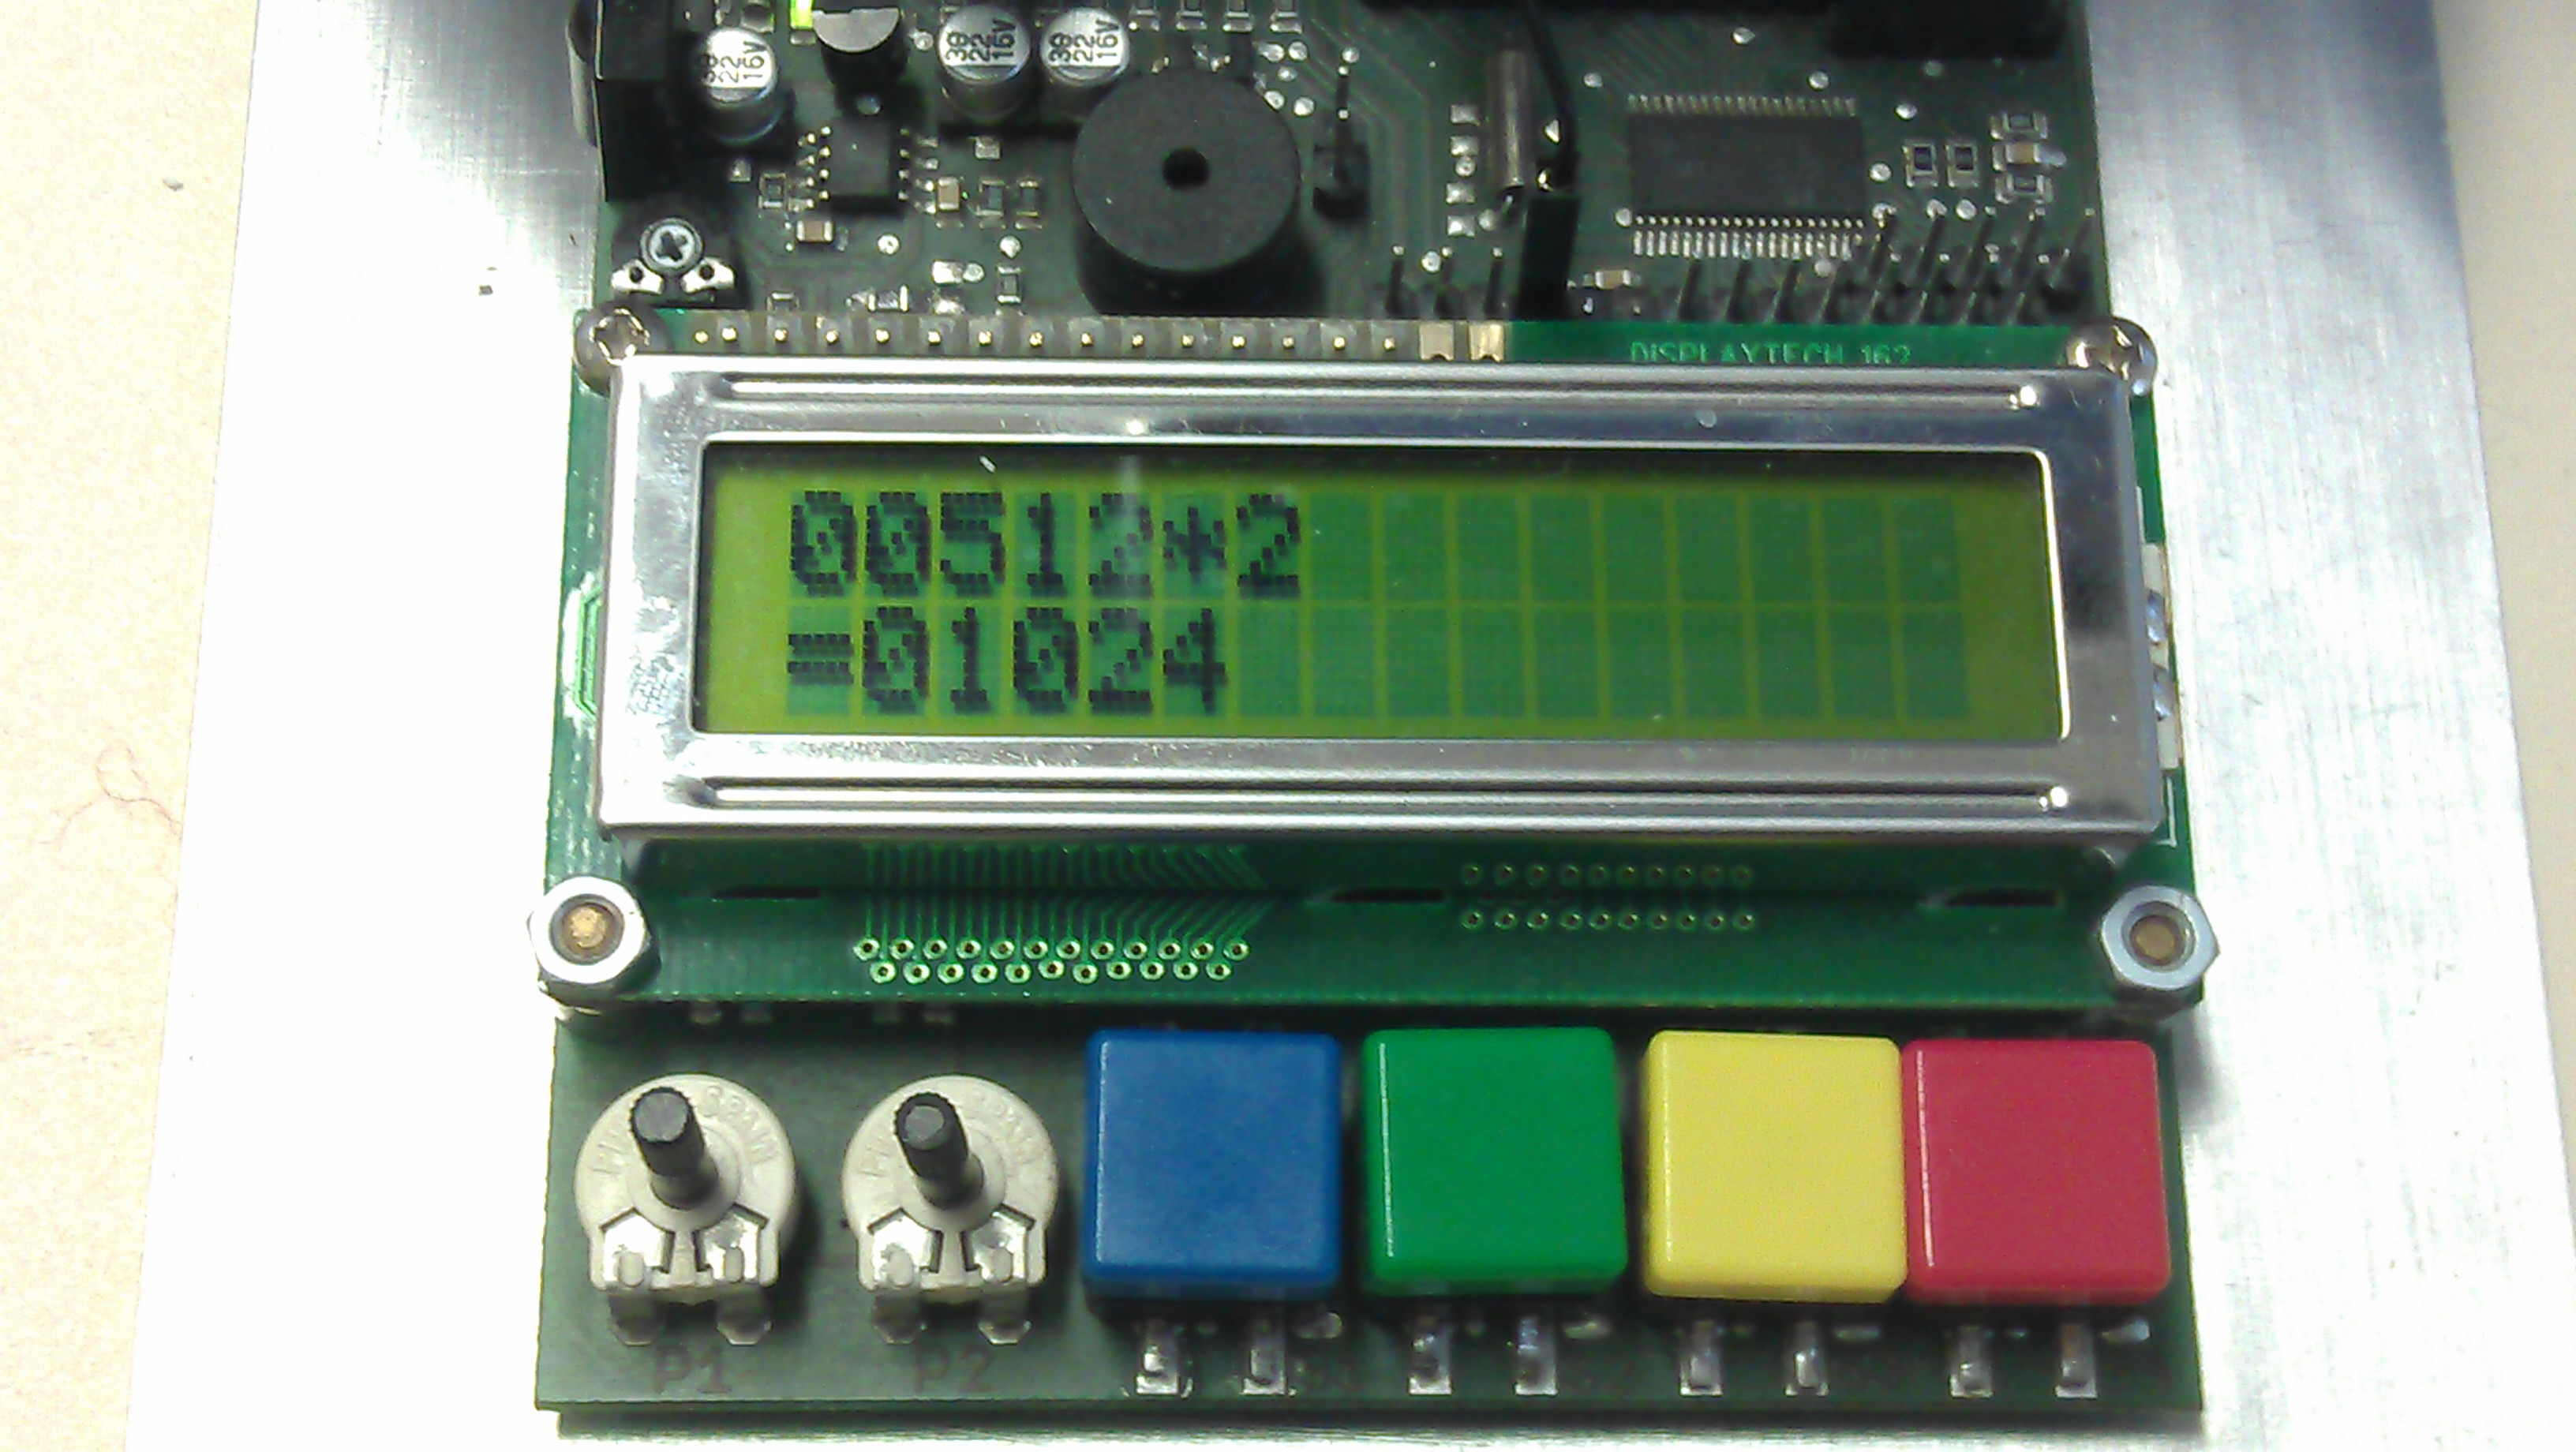
\includegraphics[width=0.7\linewidth]{img/Taschenrechner.jpg}
	\captionof{figure}[Taschenrechner]{Rechnung auf dem Taschenrechner}
	\label{fig:Taschenrechner}
\end{minipage}

Wichtig ist, dass am Ende der Interrupt-Service-Routine mit einer Warteschleife gewartet wird, da die Tasten prellen und sonst durch einen Tastendruck mehrere Interrupts ausgelöst und verarbeitet werden würden.

Das vollständige Programm kann Anhang \ref{sec:Taschenrechner} entnommen werden.

\pagebreak

\subsection{Endfassung Teatimer}
\label{VersuchTeatimer}
Bei einem Teatimer handelt es sich um ein Produkt, dass von einer vorher eingestellten Zeit sichtbar runterzählt und nach Ablauf der Zeit ein klar wahrnehmbares Signal von sich gibt.

Um dies mit dem Education Board umzusetzen, benötigt man neben dem schon bekannten LCD-Bildschirm neue Hardware: ein Timer-Modul des MSP430F2272 und ein Lautsprecher, welcher auf dem Education Board verbaut ist.


\subsubsection{Der Lautsprecher}
\label{Lautsprecher}
Der Lautsprecher lässt sich über den Pin 2.4 des MSPs ansprechen. Dieser muss dazu als Ausgangspin konfiguriert werden.
\vspace{1em}
\lstinputlisting[caption=Konfiguration von Port 2]{src/TeaTimer/LautsprecherKonfig.c}

Wird eine Spannung an den Lautsprecher angelegt, bewegt sich die Membran einmal. Durch Unterbrechen der Spannungszufuhr bewegt sich diese ein zweites Mal. Um also ein gleichmäßiges Schwingen der Membran und somit ein Ton zu erzeugen, darf immer nur kurz Spannung angelegt sein. Dies wurde mit einer For-Schleife umgesetzt: Das Bit 4 des P2OUT-Registers wird umgeschaltet und anschließend gewartet. Es entsteht ein Rechtecksignal.

\vspace{1em}
\lstinputlisting[caption=Dauerton]{src/TeaTimer/Dauerton.c}

Die Wartezeit bestimmt hierbei die Höhe des Tons. Wird kürzer gewartet, schwingt die Membran mit einer höheren Frequenz, der Ton ist höher. Wird länger gewartet, schwingt die Membran langsamer, der Ton wird tiefer.

Um nun ein Piepen zu erzeugen, muss nach einer Ton-Phase eine Pause-Phase folgen. Dies wird mit einer zweiten, äußeren Warteschleife umgesetzt.

\vspace{1em}
\lstinputlisting[caption=Piep-Funktion des Lautsprechers,label=piepen]{src/TeaTimer/Piepen.c}

Nachdem die Vorüberlegungen zu dem Umsetzen der Piep-Funktion beendet waren, galt es sich um die Timer-Mechanik Gedanken zu machen.

\subsubsection{Das Timer-Modul}
\label{TeatimerTimerA}

Der Timer des MSP430F2272 zählt Impulse aus einer spezifizierten Quelle. Beim Erreichen eines bestimmten Zählwertes löst er einen Interrupt aus. Der Teatimer soll im Sekundentakt herunterzählen. Dementsprechend muss das Timer-Modul jede Sekunde einen Interrupt auslösen, welcher dann verabeitet wird. 

Als Impulsquelle des Timer stehen mehrere Taktgeber zur Verfügung: die Auxiliary Clock, die Sub-System Master Clock, die Timer A Clock (externe Quelle) und die INCLK. Die Auxiliary Clock (kurz ACLK) wird durch einen Quarz stabilisiert und läuft mit einer Frequenz von genau 32768 Hz\footnote{MSP430Fxx2x Family User's Guide, Abschnitt 5.2.1, Seite 281}. Somit muss der Timer beim Erreichen des Zählwertes von 32768 einen Interrupt auslösen. In Listing \ref{KonfigTimer} ist diese Konfiguration dargestellt.

\vspace{1em}
\lstinputlisting[caption=Konfiguration des Timer A,label=KonfigTimer]{src/TeaTimer/KonfigTimer.c}

Damit fortlaufend in jeder Sekunde ein Interrupt ausgelöst wird, muss der Timer nach dem Erreichen des Zählwertes wieder bei 0 beginnen und erneut hochzählen. Dies wird durch den Up-Mode des Timers umgesetzt.

\vspace{1em}
\lstinputlisting[caption=Starten des Timers im Up-Mode]{src/TeaTimer/UpMode.c}

Bei Aufruf der Interrupt-Service-Routine wird jedes mal eine Variable inkrementiert. Diese repräsentiert die Anzahl der Interrupts und somit die vergangenen Sekunden seit dem Start des Timers. Daraus wird die restliche Laufzeit berechnet, welche dann auf dem LCD und mit den LEDs (sofern mit 8 LEDs möglich) dargestellt wird (siehe Abbildung \ref{fig:Teatimer}). Entspricht die vergangene Zeit der ausgewählten Startzeit, wird der Timer angehalten, die LEDs leuchten und das Piepen ertönt.

\vspace{1em}
\lstinputlisting[caption=ISR des Timers]{src/TeaTimer/ISR.c}

\vspace{1em}
\begin{minipage}{\linewidth}
	\centering
	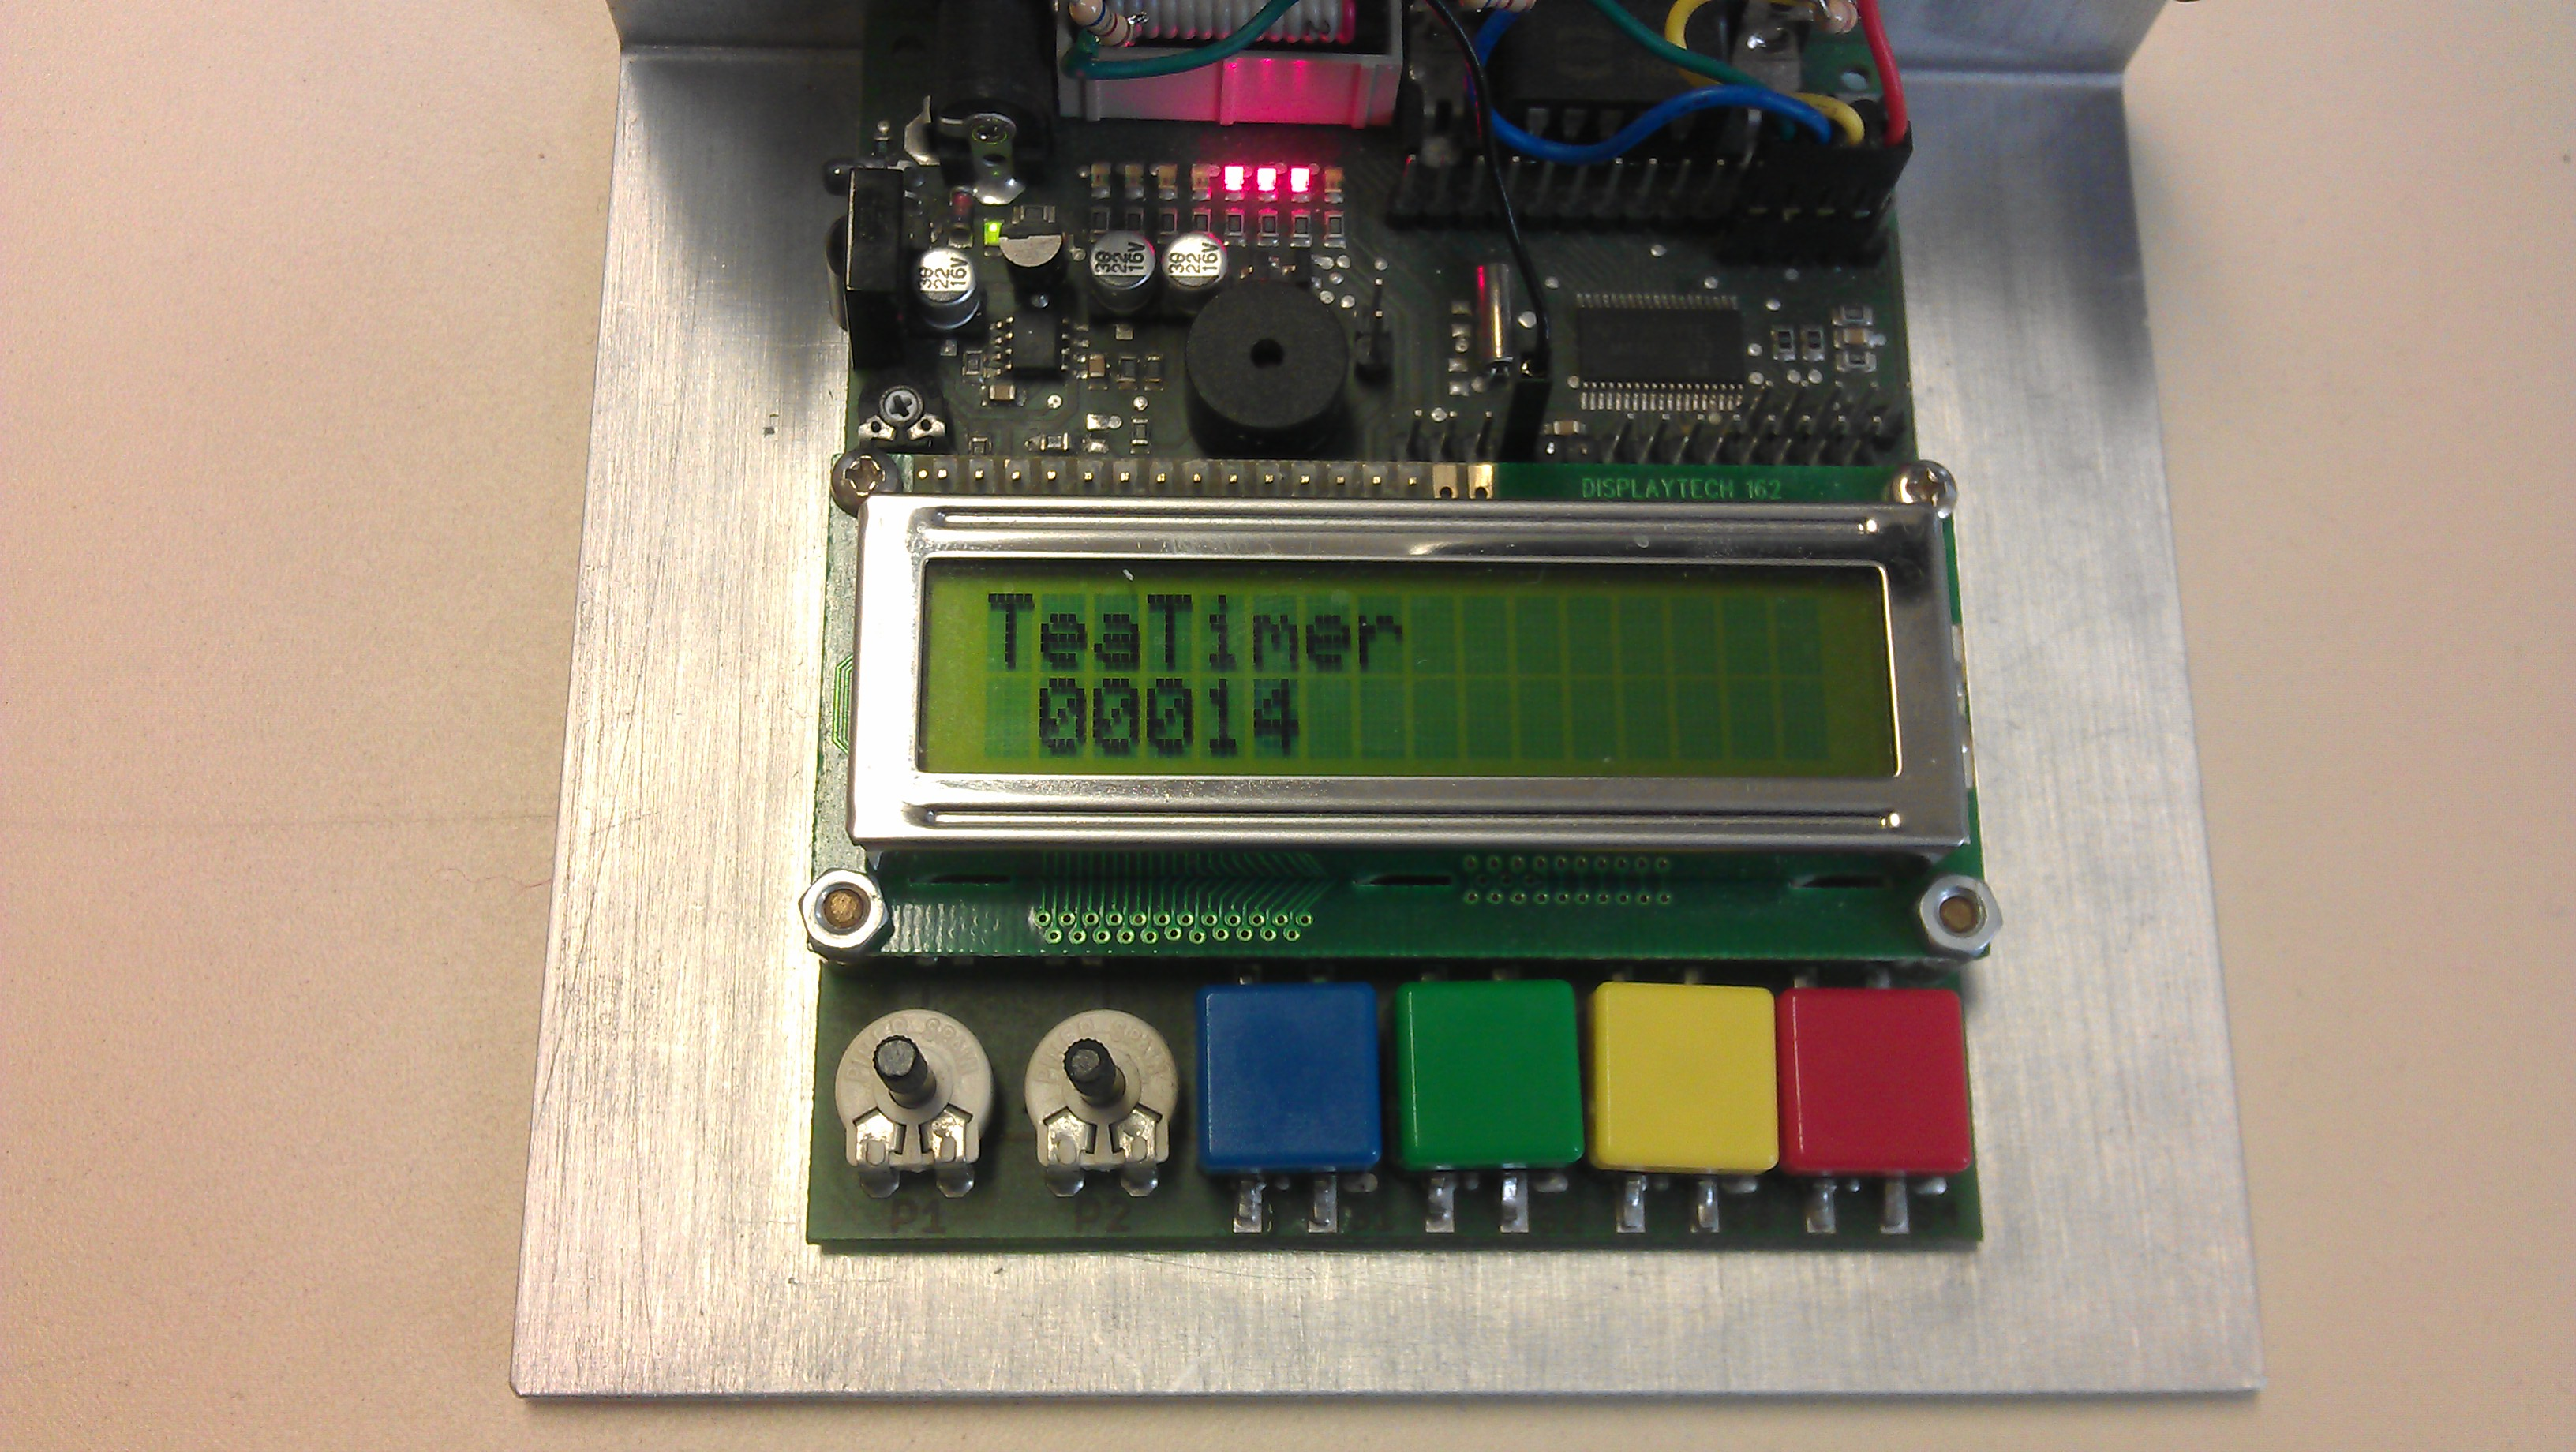
\includegraphics[width=0.7\linewidth]{img/TeaTimer2.jpg}
	\captionof{figure}[Teatimer während der Benutzung]{Teatimer in der Benutzung}
	\label{fig:Teatimer}
\end{minipage}

\vspace{1em}
Das vollständige Programm kann Anhang \ref{sec:Teatimer} entnommen werden.

\pagebreak

\subsection{Motorsteuerung}
Bei dieser Aufgabe sollte ein Motor über die Tasten des Education System Boards angesteuert werden. Der Motor kann sich nach links oder rechts drehen. An der Welle des Motors ist eine Schwungscheibe angebracht, welche mit einer schwarz-weißen Sektorenscheibe beklebt ist. Eine Reflexlichtschranke gibt bei jedem Durchgang eines hellen Sektors einen Impuls, der vom Mikrocontroller verwertet wird. Somit kann die Drehzahl ausgerechnet werden.

\vspace{1em}
\begin{minipage}{\linewidth}
	\centering
	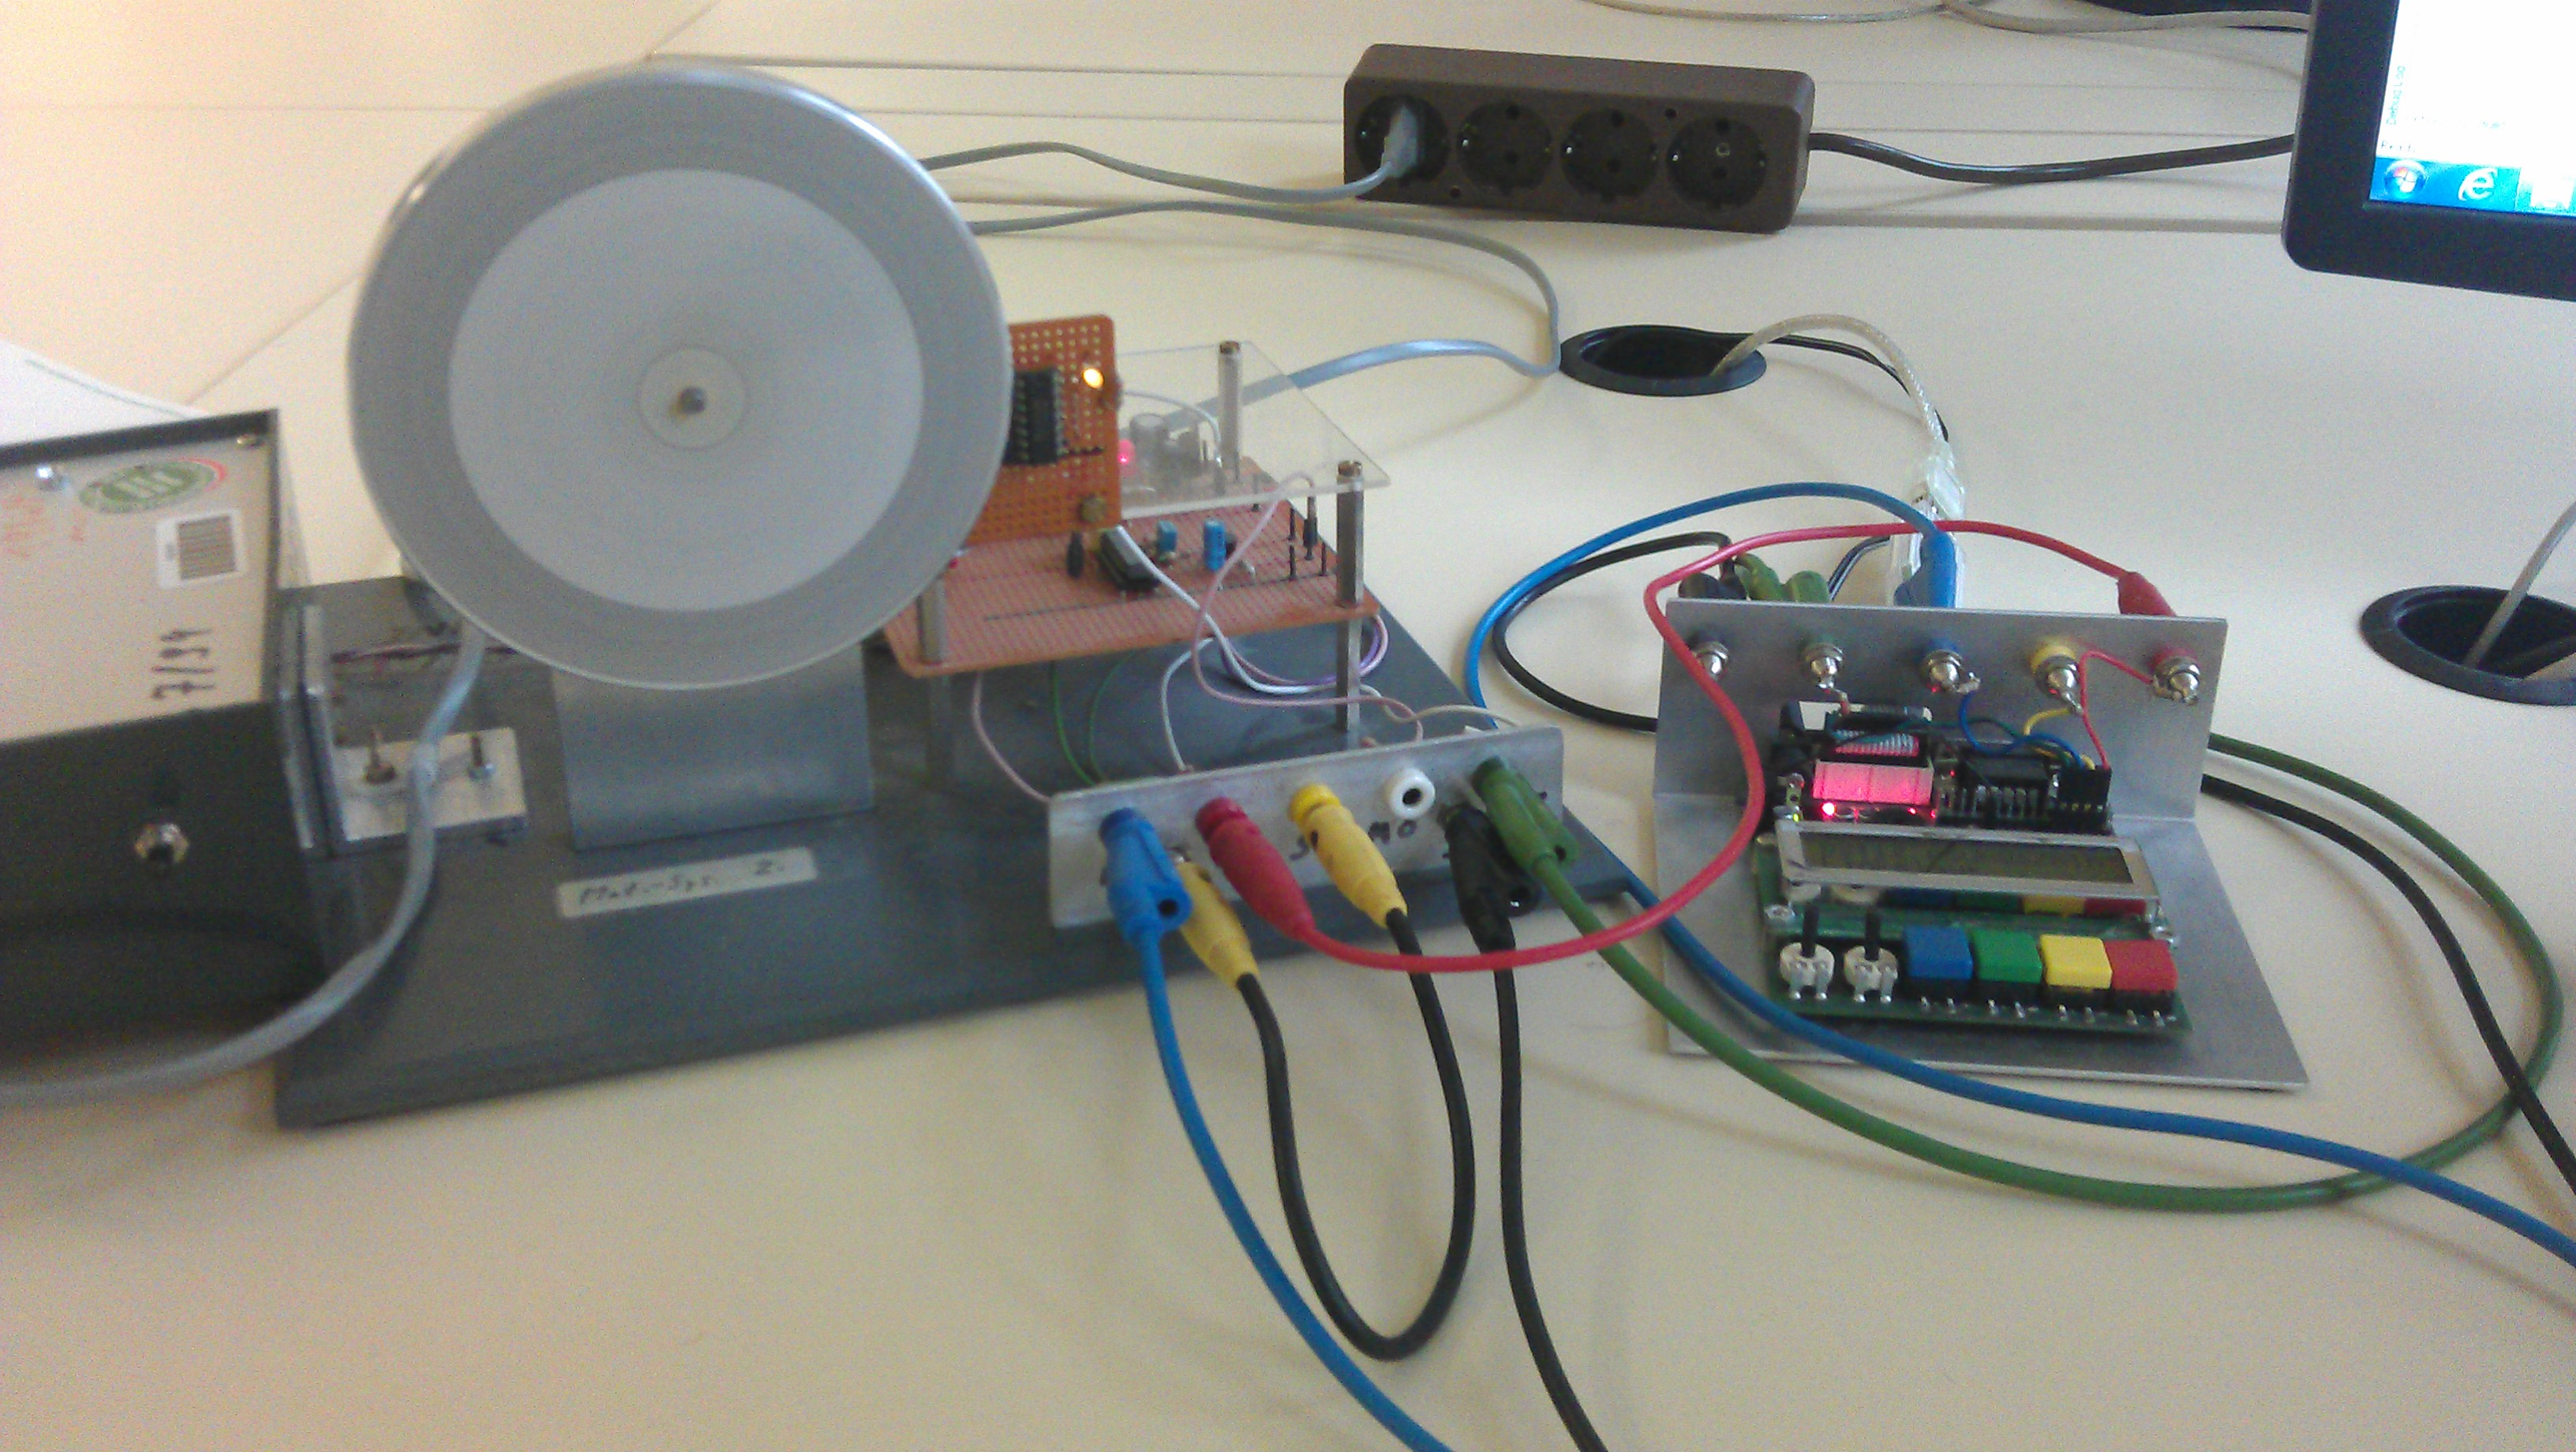
\includegraphics[width=0.7\linewidth]{img/MotorAufbau.jpg}
	\captionof{figure}[Versuchsaufbau]{Versuchsaufbau (Motor an)}
	\label{fig:MotorAufbau}
\end{minipage}

\subsubsection{Messung der Drehzahl}
Die Drehzahl soll in Umdrehungen pro Minute angegeben werden. Wie oben beschrieben wird pro Durchgang eines hellen Sektors ein Impuls durch die Reflexlichtschranke erzeugt. Die Sektorenscheibe besteht aus je 24 weißen und schwarzen Sektoren, 24 Impulse entsprechen also einer Umdrehung. Die Formel zur Berechnung der Drehzahl lautet somit: 
\[ Drehzahl = \frac{Impulse}{24*Zeit}  \]

Um die Drehzahl zu messen, gibt es zwei theoretische Ansätze:
\begin{enumerate}
	\item Es wird die Zeit zwischen zwei Impulsen gemessen. Dieser Wert wird dann auf die gewünschte Zeiteinheit hochgerechnet (z.B. eine Minute)
	\item Es wird die Anzahl der Impulse in einer festgelegten Zeitspanne gemessen (z.B. eine Sekunde) und dieser Wert wird dann auf die gewünschte Einheit hochgerechnet.
\end{enumerate}

Der Vorteil der zu erst genannten Methode ist, dass sie bei einem großen Impulsintervall sehr genaue Ergebnisse liefert. Folgen die Impulse jedoch in sehr kurzen Abständen nacheinander, ist die Genauigkeit des Ergebnisses sehr von dem Takt des Zeitgebers abhängig. Liegt dieser nah an dem Impulstakt, kommt es zu starken Rundungsfehlern. Dieses Problem hat die zweite Methode nicht, da während dem Messintervall viele Impulse eingehen und der Fehler sich herausmittelt. Dafür hat man bei einer geringen Drehzahl nur eine sehr grobe Auflösung des Ergebnisbereichs und das Ergebnis wird erst nach der festgelegten Zeitspanne aktualisiert. 

Beide Methoden haben gemeinsam, dass zwei Zähleinheiten benötigt werden. Eine misst die Zeit, die andere zählt die Impulse der Reflexlichtschranke. Hier wurde sich dafür entschieden, die zweite Methode umzusetzen, da bei dem Motor mit einer eher hohen Drehzahl zu rechnen ist.

Timer A gibt den Sekundentakt vor und wird daher wie bei der Teatimer Aufgabe konfiguriert (vgl. \ref{TeatimerTimerA}). In der Interrupt-Service-Routine wird die Drehzahl während der letzten Sekunde berechnet. Um Speicher und Zeit zu sparen, wird ausschließlich mit Integer-Variablen gearbeitet. Da bei Ganzzahldivisionen der Rest entfällt, wird bei der Rechnung erst multipliziert und dann dividiert, um ein genaueres Ergebnis zu erhalten. Außerdem werden die Faktoren gekürzt, da man sonst den Überlauf eines Registers während der Berechnung riskiert. Daraus entsteht folgende Formel: \[ Drehzahl = \frac{Impulse*5}{2}  \] Die Anzahl der Impulse sind dem Zählregister TBR des Timers B zu entnehmen, welches nach der Berechnung zurückgesetzt wird. Mit dieser Formel lässt sich eine Drehzahl von bis zu \[ \frac{2^{16}-1}{5}=13107 \] berechnen, bevor das Register während der Rechnung überläuft. 

\vspace{1em}
\lstinputlisting[caption=Interrupt-Service-Routine von Timer A,label=ISRTimerA]{src/Motorsteuerung/ISRTimerA.c}


Timer B soll die Impulse der Reflexlichtschranke zählen. Dafür muss als Impulsquelle die TBCLK angegeben werden.

\vspace{1em}
\begin{lstlisting}[caption=Konfiguration Timer B]
TBCTL = TBSSEL_0 + TBCLR; // Source Select = 0 (entspricht TBLOCK)
\end{lstlisting}

Die Reflexlichtschranke ist mit Leitung 7 von Port 4 verbunden, welche als Eingangsleitung markiert werden muss. Außerdem wird eine alternative Funktion der Leitung 4.7 genutzt, was in dem P4SEL-Register vermerkt wird.

\vspace{1em}
\begin{lstlisting}[caption=Konfiguration Port 4,label=KonfPort4]
P4DIR = ~BIT7; // P4.7 ist Eingang
P4SEL = BIT7; // Alternativfunktion wird ausgewaehlt
\end{lstlisting}

Anschließend kann der Timer B im Continuous-Mode gestartet werden. 

\vspace{1em}
\begin{lstlisting}[caption=Starten von Timer B]
TBCTL |= MC_2;
\end{lstlisting}

Somit zählt Timer B bis zu einem 16-Bit Maximalwert von \(2^{16}-1=65535\) Impulsen, bevor er automatisch wieder bei 0 mit der Zählung beginnt. Dies sollte hier allerdings nie eintreten, da laut Praktikumsleitung der Motor eine Drehzahl von 4000 Umdrehungen pro Minute nicht übersteigt. Timer A fragt jede Sekunde das Zählregister von Timer B ab und setzt es dann auf 0 zurück. Bei der genannten Geschwindigkeit werden somit in diesem Zeitintervall nur
\[4000 \frac{Umdrehungen}{Minute} * 24 \frac{Impulse}{Umdrehung}*\frac{1}{60}Minute=1600Impulse\]
von der Reflexlichtschranke an Timer B gesendet.


\vspace{1em}
\begin{minipage}{\linewidth}
	\centering
	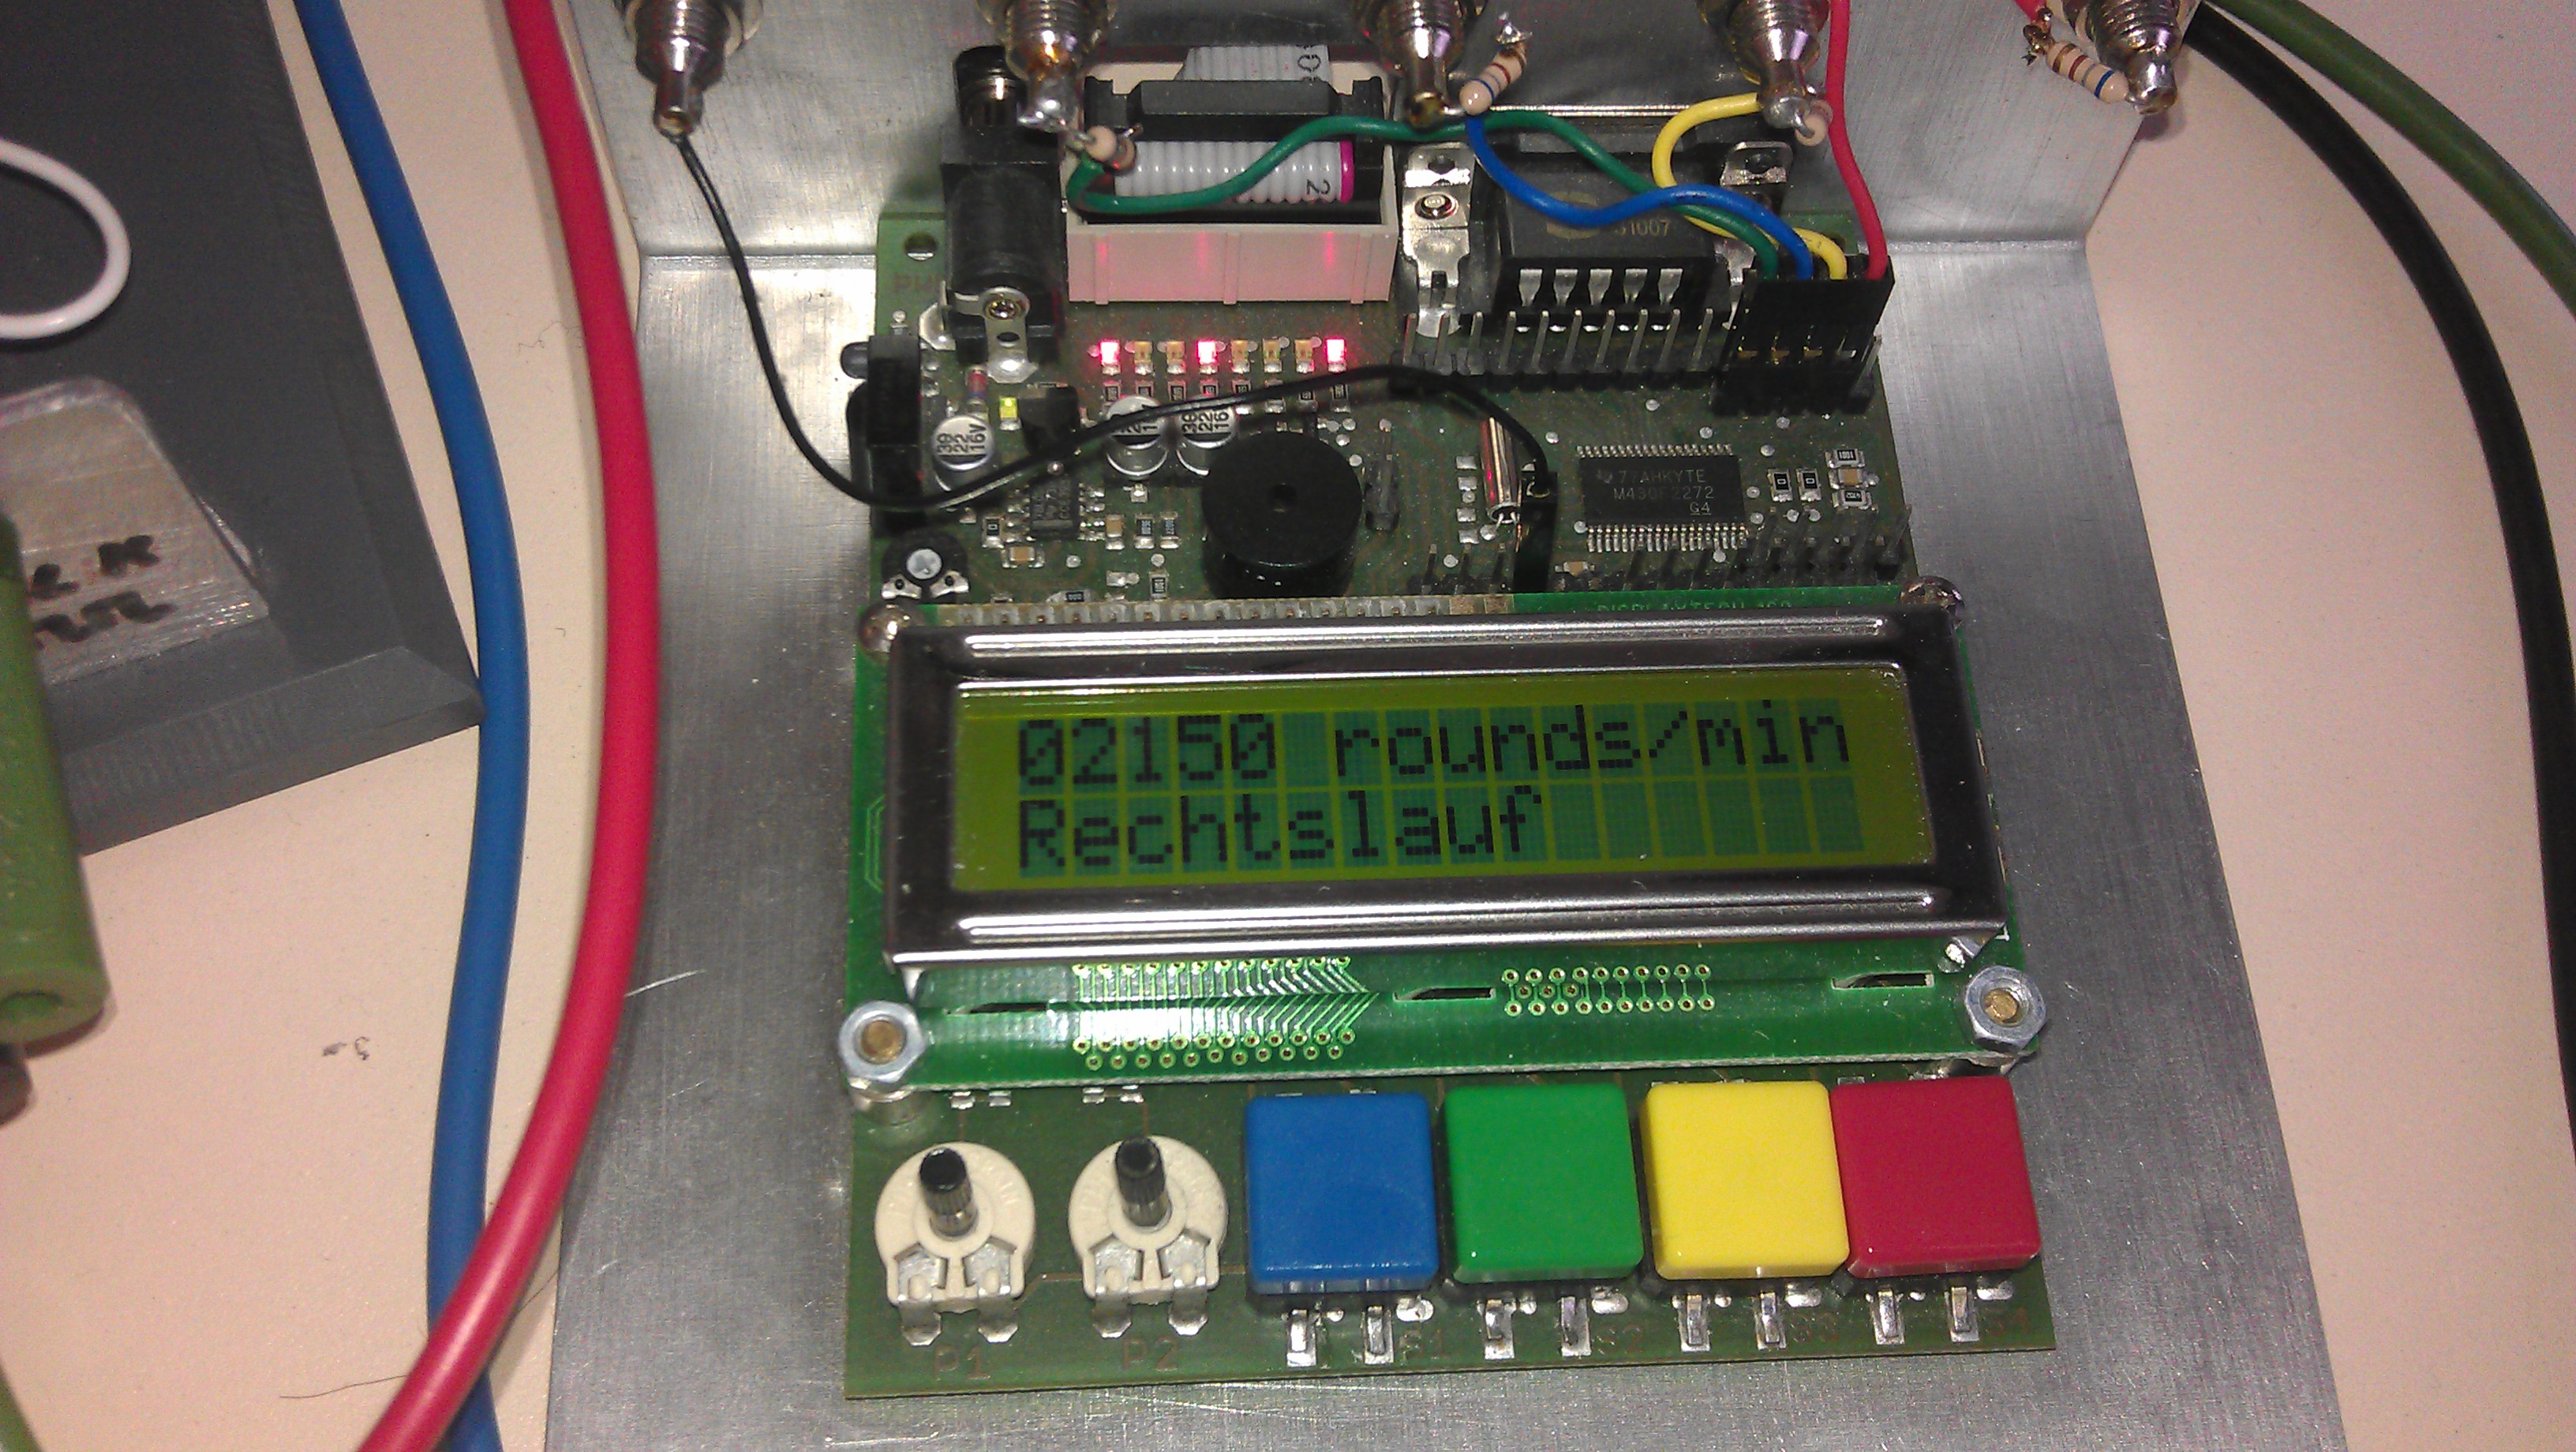
\includegraphics[width=0.7\linewidth]{img/MotorDrehzahl2.jpg}
	\captionof{figure}[Ausgabe der Drehzahl auf dem LCD-Display]{Ausgabe der Drehzahl auf dem LCD-Display}
	\label{fig:DrehzahlAusgabe}
\end{minipage}


\subsubsection{Steuerung des Motors über die Tasten}
Die Tasten werden wie im Versuch \ref{Taschenrechner} konfiguriert: Interrupts bei fallende Flanken werden für die Pins 0, 1, 2 und 5 des Ports 2 freigeschaltet.

Ein Unterschied zur Beschreibung in \ref{Taschenrechner} besteht in der Behandlung des Interrupts. Hier muss dafür gesorgt werden, dass die Tasten folgende Funktionen ausführen.

\begin{table}[h]
	\begin{centering}
		\begin{tabular}{|c|c|c|c|}
			\hline 
			\textbf{Port} & \textbf{Taster} & \textbf{Farbe} & \textbf{Funktion}\tabularnewline
			\hline 
			\hline 
			P2.0 & S1 & rot & Motor anhalten\tabularnewline
			\hline 
			P2.1 & S2 & gelb & ohne Funktion\tabularnewline
			\hline 
			P2.2 & S3 & grün & Motor im Rechtslauf starten\tabularnewline
			\hline 
			P2.5 & S4 & blau & Motor im Linkslauf starten\tabularnewline
			\hline 
		\end{tabular}
		\par\end{centering}
	\smallskip{}
	\protect\caption{Tasterzuordnung}
\end{table}

Der Motor ist über die Leitungen 4 und 6 des Port 2 ansteuerbar. Die Konfiguration dafür wurde schon in Listing \ref{KonfPort4} durchgeführt, indem diese Leitungen als Ausgangsleitung vermerkt wurden.
Soll der Motor im Linkslauf starten, muss P4.6 angesteuert werden, während P4.4 kein Strom bekommt. Für den Rechtslauf sind die Leitungen umgekehrt anzusteuern. Um den Motor zu stoppen, wird beiden Leitungen die Stromzufuhr entzogen. Dies führt zur folgender Interupt-Service-Routine:

\vspace{1em}
\lstinputlisting[caption=Interrupt-Service-Routine der Tasten]{src/Motorsteuerung/ISRTasten.c}

Das vollständige Programm kann Anhang \ref{sec:Motorsteuerung} entnommen werden.

\pagebreak

\subsection{Fernbedienung}
Bei dieser abschließenden Aufgabe soll mit einer Philips-RC5 codierten Fernbedienung ein Teatimer bedient werden können. Dies lässt sich in zwei Teilaufgaben aufteilen:
\begin{enumerate}
	\item Telegramme der Fernbedienung empfangen und auswerten
	\item Teatimer bedienen
\end{enumerate}

\subsubsection{Telegramme empfangen und auswerten}
Die Fernbedienung sendet Infrarot-Impulse, die von einem Infrarot-Empfängerbaustein des Education Systems empfangen werden können. Diese Infrarot-Impulse codieren einzelne Bits, indem die Impulse in verschiedenen Zeitabständen erscheinen und verschieden lange anhalten. Der Empfängerbaustein drückt den Ruhezustand (kein Infrarotlicht) durch ein HIGH auf seiner Leitung aus. Eine 1 wird durch eine fallende Flanke ausgedrückt, also ein Wechsel von kein Impuls zu einem Impuls. Um mehrere 1 nacheinander zu versenden, sind steigende Hilfsflanken nötig, um wieder fallende Flanken erzeugen zu können. Um die Hilfsflanken von informationstragenden Flanken unterscheiden zu können, sind die Impulse getaktet (siehe Abbildung \ref{fig:Infrarot}). Informationstragende Flanken treten in einem Intervall von \(888{\mu}s*2=1776{\mu}s\) auf.

\vspace{1em}
\begin{minipage}{\linewidth}
	\centering
	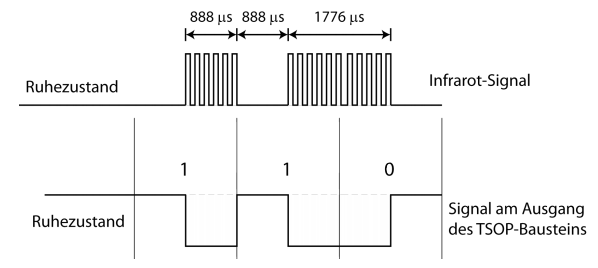
\includegraphics[width=1\linewidth]{img/Infrarot.png}
	\captionof{figure}[Empfang von einem Infrarot-Signal am Empfängerbaustein]{Empfang von einem Infrarot-Signal am Empfängerbaustein\footnotemark}
	\label{fig:Infrarot}
\end{minipage}

\footnotetext{{Quelle: \url{https://homepages.thm.de/~hg6458/mpt-Dateien/MPTP.pdf}, Seite 37}}

Um ein Telegramm der Fernbedienung auswerten zu können, muss also die Zeit zwischen zwei Flanken gemessen werden. Ein Telegramm startet immer mit einer 1, also einer fallenden Flanke. Hat das nächste Datum den gleichen Wert, folgt eine steigende Hilfsflanke nach einem kurzen Intervall (\(888{\mu}s\)), gefolgt von der informationstragenden Flanke nach weiteren \(888{\mu}s\). Wird als nächstes jedoch eine 0 gesendet, ist keine Hilfsflanke nötig um eine steigende Flanke darzustellen, die nächste Flanke folgt also nach einem langen Intervall (\(1776{\mu}s\)).

Um diese Methodik umsetzen zu können, muss zu erst der Empfängerbaustein konfiguriert werden. Dieser ist über die Leitung 3 des Port 2 mit dem MSP430 verbunden. Empfängt dieser eine fallende Flanke soll er ein Interrupt auslösen. Da nach einer fallenden Flanke immer eine steigende folgt, muss später in der Interrupt Service Routine das Bit 3 des P2IES-Registers umgeschaltet werden.

\vspace{1em}
\begin{lstlisting}[caption=Konfiguration Port 2]
P2IE = BIT3;     // Interrupt Enable an Leitung 3
P2IES = BIT3;		// Interrupt fuer fallende Flanke
\end{lstlisting}

Um die Zeit zwischen den Flanken zu messen, wird der Timer A des MSP430F2272 verwendet. Dieser bezieht seinen Takt von der Auxiliary Clock. Er wird im Continuous-Mode gestartet, zählt also solange hoch, bis der Maximalwert des Registers erreicht wird.

\vspace{1em}
\begin{lstlisting}[caption=Konfiguration Timer A]
TACTL = TASSEL_1 + TACLR;
TACTL |= MC_2; // Continuous-Mode
\end{lstlisting}

In der Interrupt-Service-Routine des Infrarot-Empfängerbausteins kann nun die Zeit seit der letzten Flanke, also seit dem letzten Interrupt, ausgewertet und in ein konkretes Datum umgewandelt werden. Wie oben erklärt, startet das Telegramm zu einem unbekannten Zeitpunkt mit einer 1. Der Zählwert des Timer-Registers kann hier also jeden Wert annehmen und wird daher nicht beachtet. Das Register wird auf 0 zurückgesetzt. Der nächste Wert ist jedoch relevant. Eine kleiner Wert bedeutet, dass wieder eine 1 gesendet wurde, ein großer Wert bedeutet, dass eine 0 gesendet wurde. Doch was ist ein großer oder ein kleiner Wert? Die Zeitgeber-Einheit zählt Impulse in einer Frequenz von 32768 Hz, also ein Impuls alle \(30.52{\mu}s\). Bei einem kurzen Intervall von \(888{\mu}s\) müsste somit ein Zählwert von ca. \(888{\mu}s/30.52{\mu}s\approx29\) in dem Register des Timer As stehen, bei einem langen Intervall dementsprechend der doppelte Wert von ca. 58. Um Messfehler und Rundungsungenauigkeiten zu beseitigen, wird jeweils eine Abweichung von bis zu 10 erlaubt, um dem Messwert ein Datum zu zuordnen. Nachdem ein Datum ausgewertet wurde, wird der Wert in ein Feld gespeichert. Folgender Ausschnitt aus der ISR setzt dieses Verhalten um:

\vspace{1em}
\begin{lstlisting}[caption=Auswertung des Impulsintervalls]
-- globale Variablen ---
int dateCounter = 0; // zaehlt Elemente des aktuellen Telegramms
int slowFlank = 58; // berechneter Wert fuer langes Intervall
int fastFlank = 29; // berechneter Wert fuer kurzs Intervall
int message[14]; // speichert Bits des Telegramms
int bitValue = 1; // Wert des letzten Datums
int hilfsFlanke = 0; // gibt an, ob letzte Flanke informationstragend war

-- in der ISR --- 
int timerAReg = TAR;
TAR = 0; // Register zuruecksetzen

/* langsame Flanke */
if (timerAReg<slowFlank + 10 && timerAReg>slowFlank - 10) {
	bitValue ^= 1; 
	message[dateCounter++] = bitValue; 
	hilfsFlanke = 0; 
}
/* schnelle Flanke */
else if (timerAReg<fastFlank + 10 && timerAReg>fastFlank - 10) {
	// letzte Flanke war informationstragend, dies ist eine Hilfsflanke
	if (hilfsFlanke == 0) {
	hilfsFlanke = 1;
	}
	// letzte Flanke war Hilfsflanke, diese ist informationstragend
	else {
		message[dateCounter++] = bitValue;
		hilfsFlanke = 0; // war keine HilfsFlanke
	}
}
else {
	/* Zaehlwert liegt ausserhalb der definierten Werte, muss daher der Anfang eines neuen Telegramms sein */
	dateCounter = 0;
	bitValue = 1;
	message[dateCounter++] = bitValue;
}
P2IES = P2IES ^ BIT3; // EdgeSelect umschalten
\end{lstlisting}

Ein Telegramm besteht aus insgesamt 14 Bits. Wie aus Abbildung \ref{fig:TelegrammCode} zu entnehmen ist, stellen die letzten 6 Bits das Kommando dar.



\vspace{1em}
\begin{minipage}{\linewidth}
	\centering
	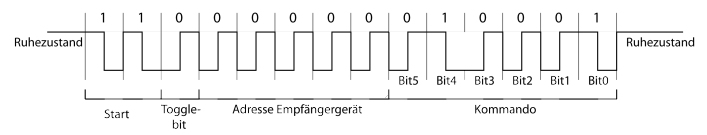
\includegraphics[width=1.1\linewidth]{img/Telegramm.png}
	\captionof{figure}[Beispiel eines RC5-Telegramms]{Beispiel eines RC5-Telegramms\footnotemark}
	\label{fig:TelegrammCode}
\end{minipage}
\footnotetext{Quelle: \url{https://homepages.thm.de/~hg6458/mpt-Dateien/MPTP.pdf}, Seite 38}

Durch sukzessives Linksshiften und Addieren lässt sich leicht aus den 6 Bits die Kommando-Nummer berechnen.

\vspace{1em}
\begin{lstlisting}[caption=Berechnung der Kommando-Nummer]
for (char i=8; i < telegrammSize; i++) {
	kommando = kommando << 1;
	kommando += message[i];
}
\end{lstlisting}


Jeder Taste der Fernbedienung ist genau eine Kommando-Nummer zugewiesen:

\begin{table}[h]
	\centering
	
	
	\begin{tabular}{|c|c|c|c|c|}
		\cline{1-2} \cline{4-5}
		\textbf{Taste}                                   & \textbf{Tastencode} & \multicolumn{1}{l|}{} & \textbf{Taste}                        & \textbf{Tastencode} \\ \cline{1-2} \cline{4-5} \noalign{\smallskip} \cline{1-2} \cline{4-5}
		\cellcolor[gray]{.8}0 						 & 0                   &                       & \cellcolor[gray]{.8}Ch+           & 22                  \\ \cline{1-2} \cline{4-5} 
		\cellcolor[gray]{.8}1                        & 1                   &                       & \cellcolor[gray]{.8}Ch-           & 21                  \\ \cline{1-2} \cline{4-5} 
		\cellcolor[gray]{.8}2                        & 2                   &                       & \cellcolor[gray]{.8}TV/AV         & 56                  \\ \cline{1-2} \cline{4-5} 
		\cellcolor[gray]{.8}3                        & 3                   &                       & \cellcolor[gray]{.8}Standby       & 12                  \\ \cline{1-2} \cline{4-5} 
		\cellcolor[gray]{.8}4                        & 4                   &                       & \cellcolor[gray]{.8}Smart Picture & 13                  \\ \cline{1-2} \cline{4-5} 
		\cellcolor[gray]{.8}5                        & 5                   &                       & \cellcolor[gray]{.8}Smart Sound   & 36                  \\ \cline{1-2} \cline{4-5} 
		\cellcolor[gray]{.8}6                        & 6                   &                       & \cellcolor[gray]{.8}Favorite      & 34                  \\ \cline{1-2} \cline{4-5} 
		\cellcolor[gray]{.8}7                        & 7                   &                       & \cellcolor[gray]{.8}Mute          & 13                  \\ \cline{1-2} \cline{4-5} 
		\cellcolor[gray]{.8}8                        & 8                   &                       & \cellcolor[gray]{.8}Menu          & 18                  \\ \cline{1-2} \cline{4-5} 
		\cellcolor[gray]{.8}9                        & 9                   &                       & \cellcolor[gray]{.8}ok            & 47                  \\ \cline{1-2} \cline{4-5} 
		\cellcolor[gray]{.8}Vol+                     & 16                  &                       & \cellcolor[gray]{.8}Display       & 15                  \\ \cline{1-2} \cline{4-5}
		\cellcolor[gray]{.8}Vol-                     & 17                  &                       & \cellcolor[gray]{.8}A/Ch	       & 23                  \\ \cline{1-2} \cline{4-5}  
		\cellcolor[gray]{.8}Sleep                    & 35                  & \multicolumn{1}{l|}{} & \cellcolor[gray]{.8}MTS           & 44                  \\ \cline{1-2} \cline{4-5} 
	\end{tabular}
	\caption{Tastencodes der Fernbedienung Philips RC1152605}
	\label{TastencodeTabelle}
\end{table}

Die Fernbedienung wiederholt das Senden des Telegramms in einem Abstand von 100 ms solange die Taste auf der Fernbedienung gedrückt wird. Damit man erkennen kann, ob es sich um ein wiederholtes oder ein neues Telegramm handelt, gibt es das Togglebit (siehe Abbildung \ref{fig:TelegrammCode}). Dieses ändert nach jedem Tastendruck seinen Wert. Wiederholte Telegramme haben also alle den gleichen Wert an dieser Bit-Stelle.

Sobald alle 14 Bits eines Telegramms empfangen wurden und das neue Togglebit sich von dem des letzten ausgewerteten Telegramms unterscheidet, kann das neue Kommando ausgeführt werden.

\vspace{1em}
\begin{minipage}{\linewidth}
	\centering
	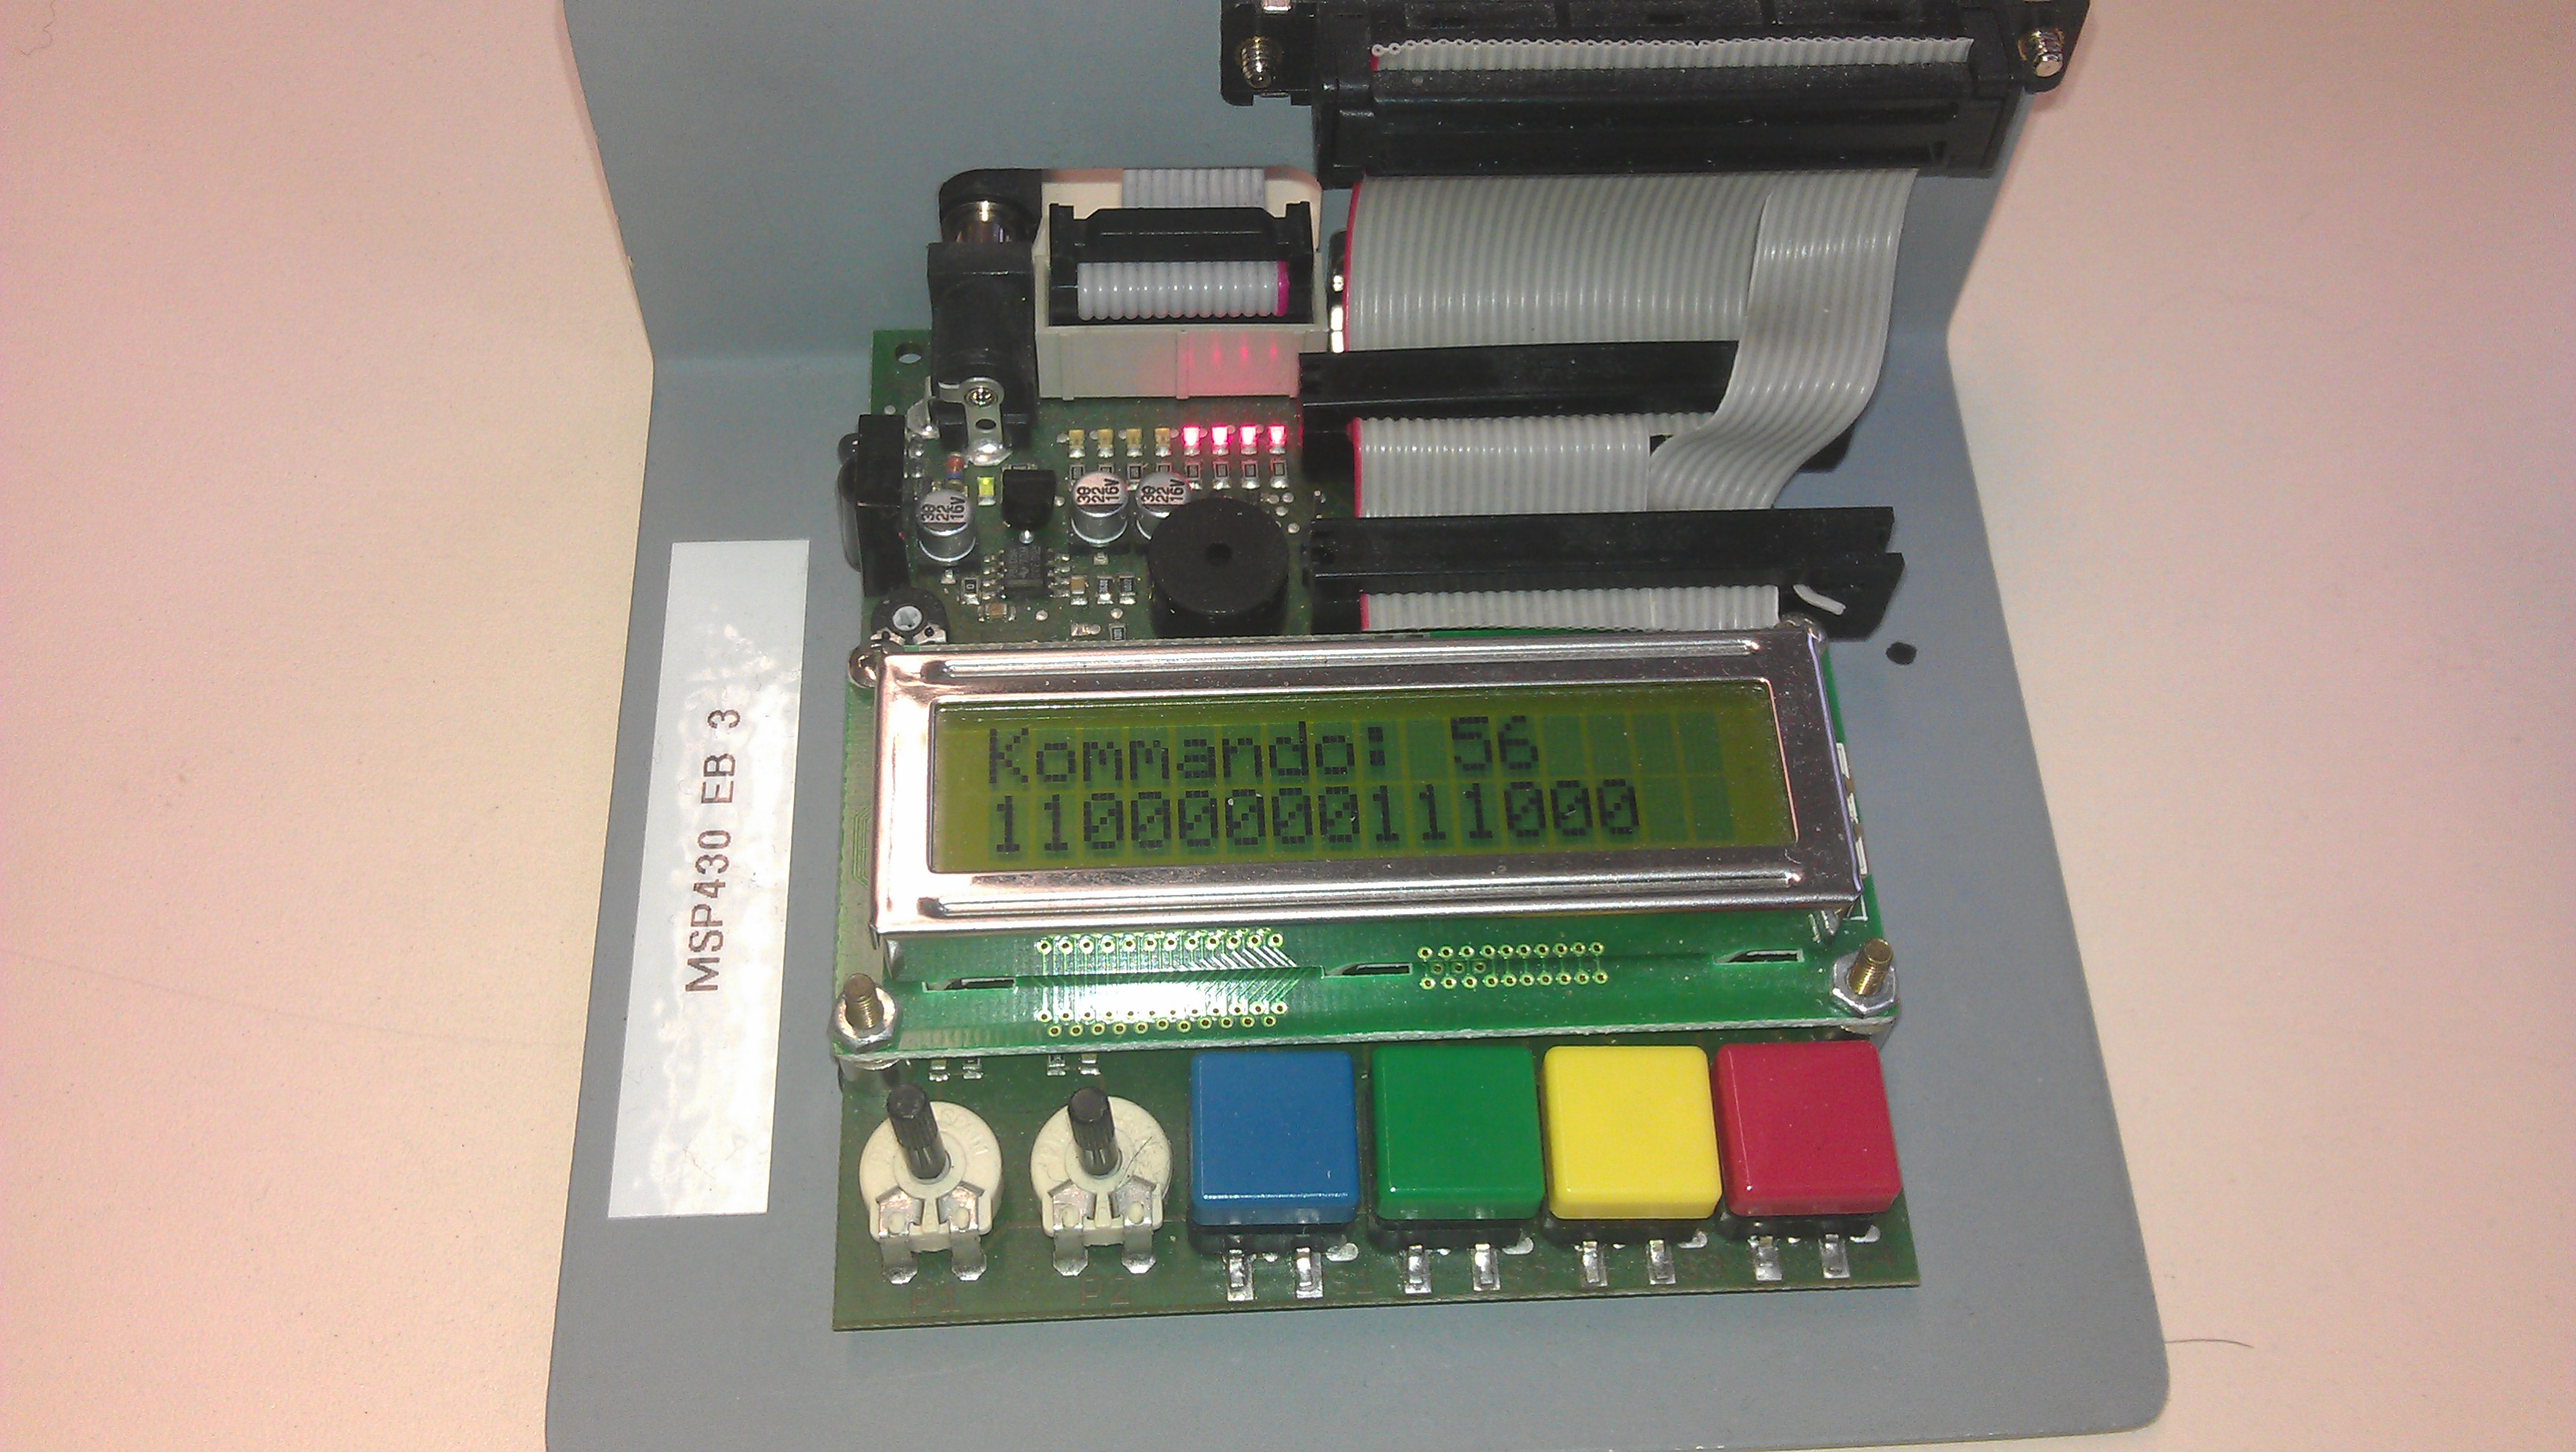
\includegraphics[width=0.7\linewidth]{img/Fernbedienung2.jpg}
	\captionof{figure}{Telegramm wurde ausgewertet und Kommando erkannt}
	\label{fig:Kommando}
\end{minipage}

\subsubsection{Kommando ausführen und Teatimer bedienen}
Nachdem es nun möglich ist, Kommandos über die Fernbedienung zu erhalten, müssen diese an die Steuerung eines Teatimer gekoppelt werden. Die grundlegenden Funktionen und der Aufbau eines Teatimers sind bei der Aufgabe \ref{VersuchTeatimer} aufgeführt.\newline
Es wurde eine Zustandsmaschine entworfen, welche die einzelnen Aktionen nach Erhalt eines Kommandos festlegt.

\vspace{1em}
\begin{minipage}{\linewidth}
	\centering
	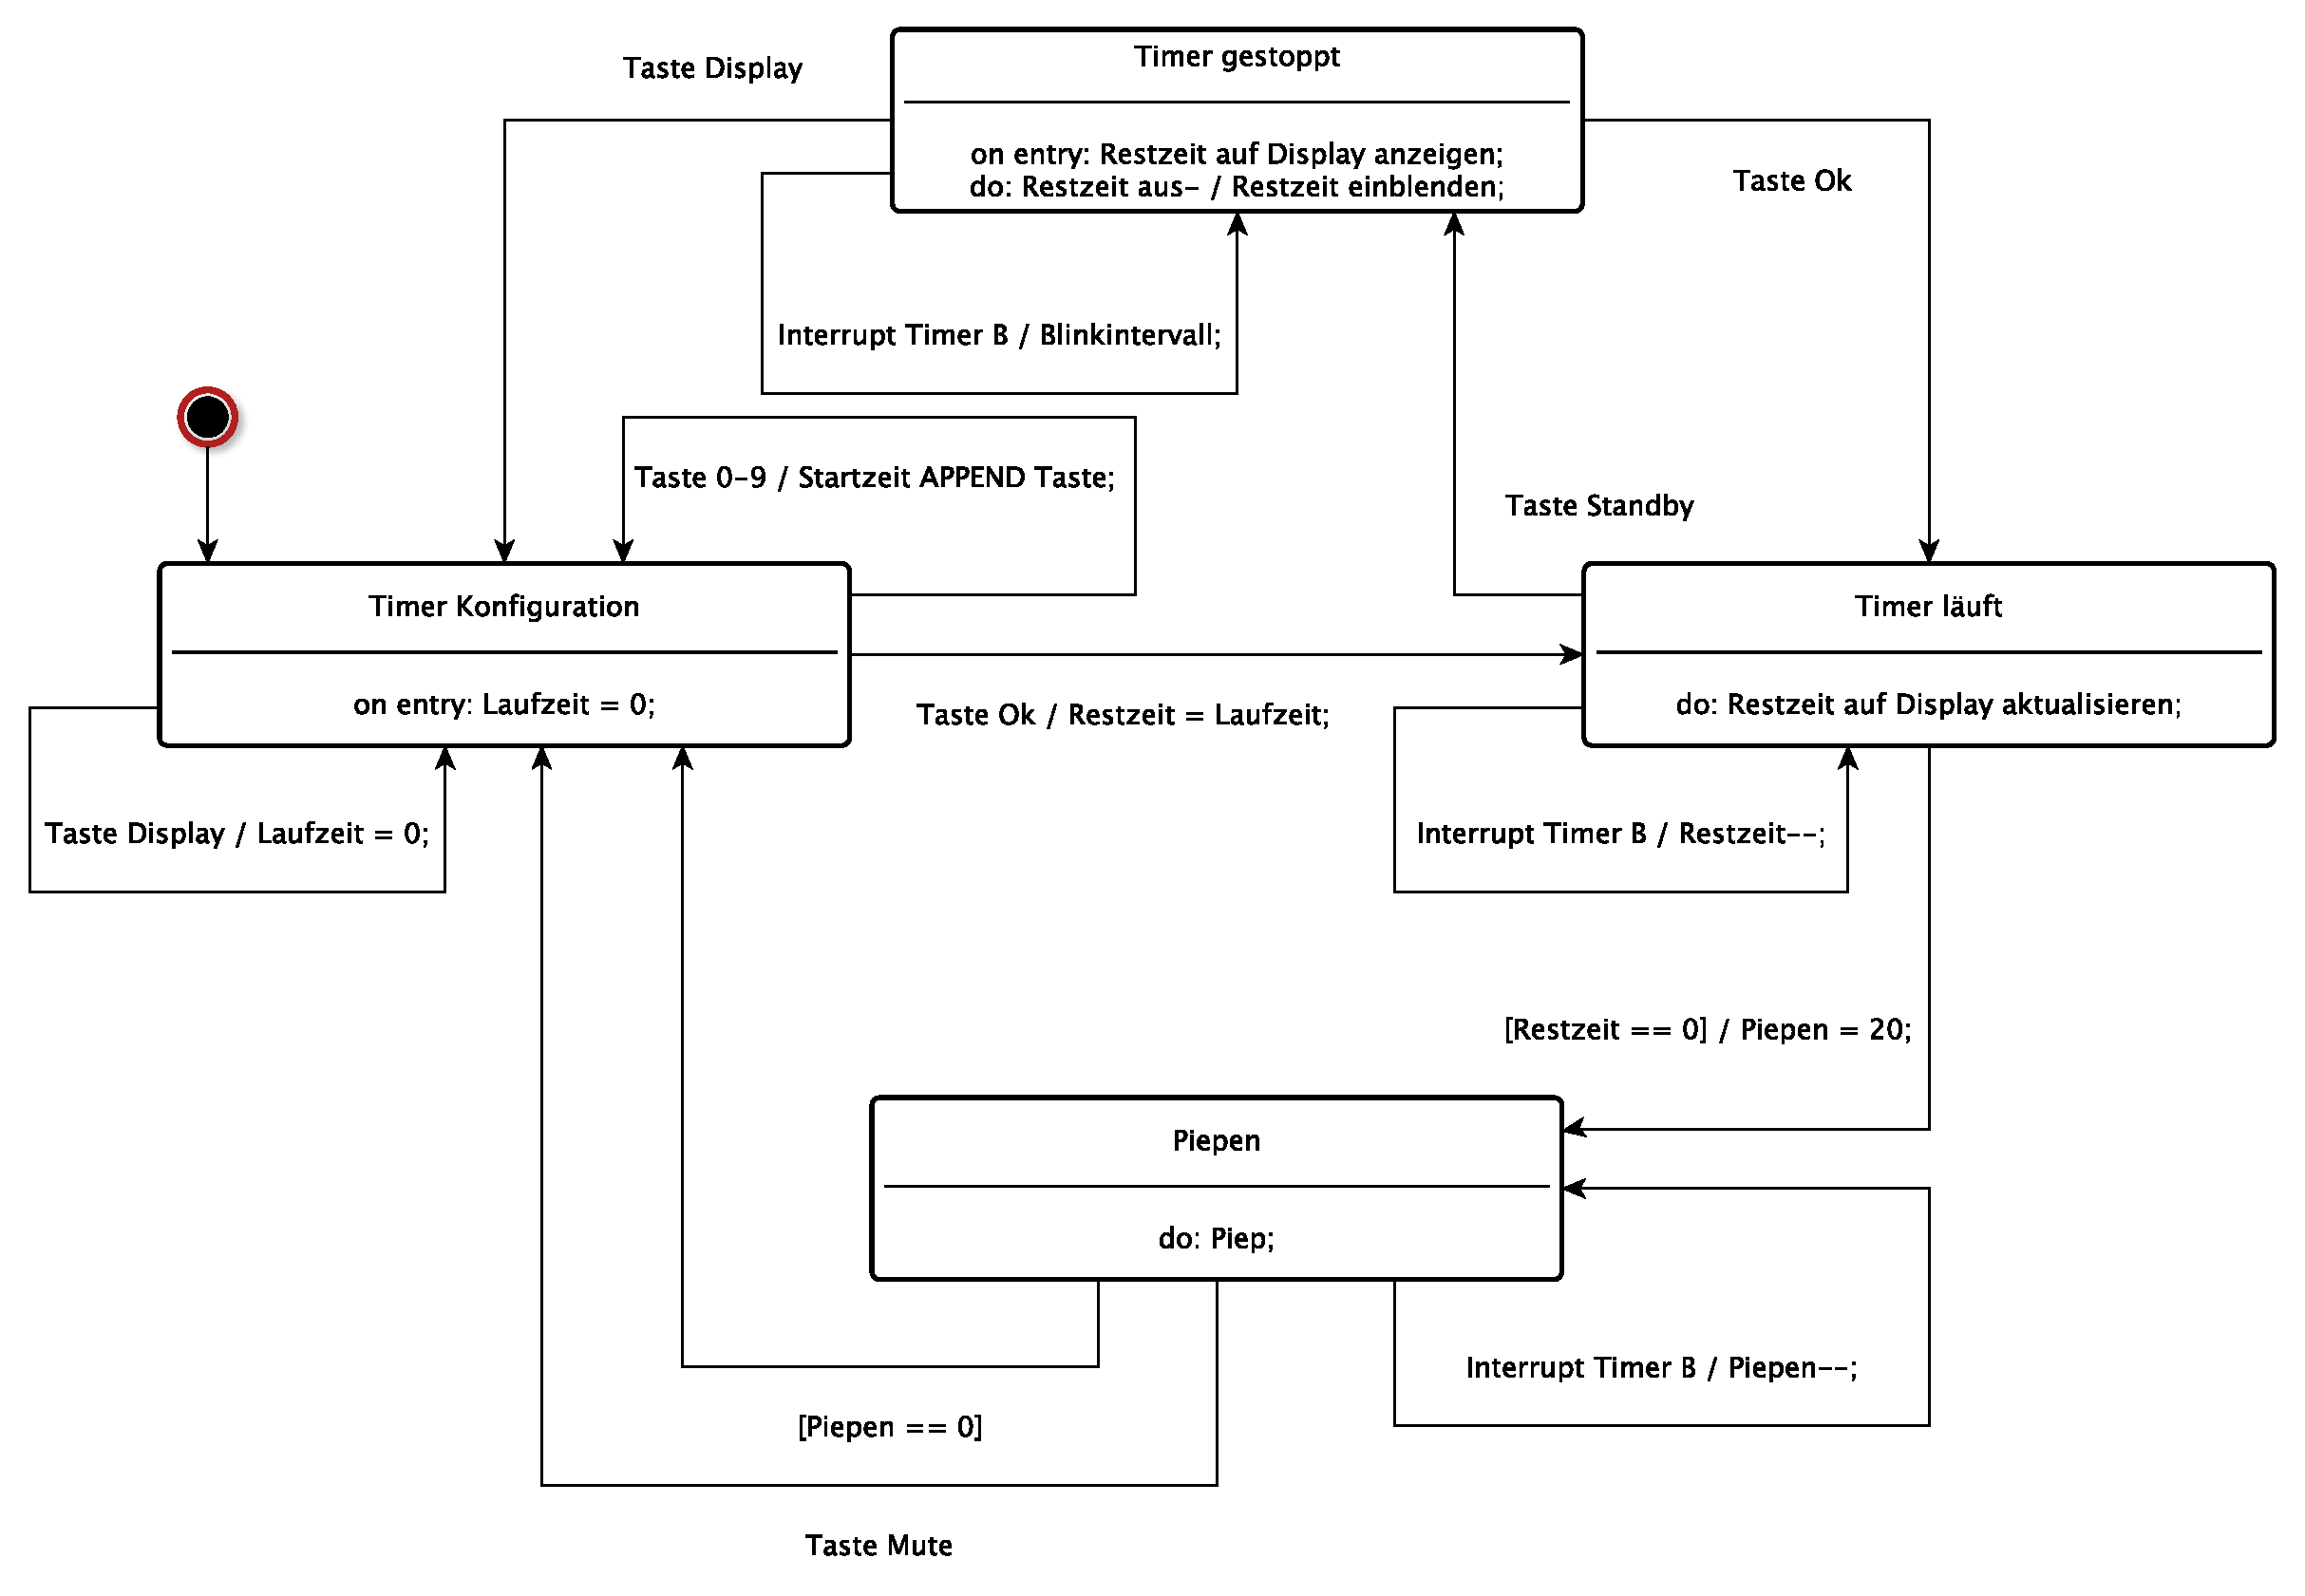
\includegraphics[width=1\linewidth]{img/Zustandsdiagramm.pdf}
	\captionof{figure}{Zustandsautomat des Teatimers}
	\label{fig:StateMachine}
\end{minipage}

Wie der Abbildung \ref{fig:StateMachine} zu entnehmen ist, gibt es vier Zustände in denen sich der Teatimer befinden kann. Die Auswirkung der Zustände teilt sich in drei Aspekte auf:
\begin{itemize}
	\item Was passiert, wenn in einen Zustand überführt wird?
	\item Wie verhält sich das Timer-Modul in diesem Zustand?
	\item Welche Tasten der Fernbedienung können in diesem Zustand verwendet werden?
\end{itemize}

Nach diesen Punkten werden im folgenden die einzelnen Zustände beschrieben:

\textbf{Konfiguration}
\begin{lstlisting}
#define KONFIG  0
\end{lstlisting}
In diesem Zustand startet der Teatimer. Das Timer-Modul arbeitet nicht und wird daher angehalten. Eine eventuell vorher eingestellte Zeit wird auf 0 gesetzt. Über die Ziffer-Tasten der Fernbedienung kann eine neue Zeit eingestellt werden. Dabei wird die durch eine Taste dargestellte Ziffer der aktuellen Zeit hinten angehängt, bis zu einem Maximalwert von 65535. Die Taste \glqq Display\grqq{} setzt die eingestellte Zeit auf 0 zurück. Mit der Taste \glqq OK\grqq{} wird der Teatimer gestartet und somit in den Zustand \glqq Laufend\grqq{} überführt.

\textbf{Timer läuft}
\begin{lstlisting}
#define RUNNING  1
\end{lstlisting}
Der Timer wird so konfiguriert, dass er jede Sekunde einen Interrupt auslöst, und anschließend gestartet. Bei jedem Interrupt wird die Restzeitanzeige auf dem Display aktualisiert. Ist die Zeit abgelaufen, oder wenn als Startwert 0 ausgewählt wurde, geht der Teatimer in den Zustand \glqq Piepen\grqq{} über. Wird während der Laufzeit des Timers die \glqq Standby\grqq{}-Taste betätigt, hält der Teatimer an und befindet sich somit im Zustand \glqq Gestoppt\grqq{}.

\textbf{Timer gestoppt}
\begin{lstlisting}
#define STOPPED  2
\end{lstlisting}
In diesem Zustand soll das Display mit der Restanzeige blinken. Dafür wird ebenfalls das Timer-Modul genutzt, welches nun im halben Sekundentakt ein Interrupt auslöst. Hier wird nicht mehr die restliche Zeit runtergezählt und dargestellt, sondern abwechselnd die Restzeit und eine \glqq - - - -\grqq{}-Ausgabe gezeigt. Es gibt zwei Möglichkeiten, diesen Zustand zu verlassen. Entweder wird der Teatimer über die Taste \glqq OK\grqq{} wieder gestartet und in den Zustand \glqq Laufend\grqq{} versetzt oder man setzt ihn mit der Taste \glqq Display\grqq{} in den Konfigurationsmodus zurück.

\textbf{Timer piept}
\begin{lstlisting}
#define BEEPING  3
\end{lstlisting}
Dieser Zustand wird durch den Ablauf der Zeit erreicht. Durch den Timer und den Lautsprecher (vgl. \ref{Lautsprecher}) wird jede Sekunde ein Doppel-Piepen erzeugt. Nach 5 Piep-Signalen oder durch Betätigen der \glqq Mute\grqq{}-Taste wird der Teatimer wieder in den Konfigurationsmodus überführt.



Diese Funktionalitäten werden durch drei verschiedene Funktionen im Code umgesetzt. Hierbei wurden die Tastencodes, wie sie in der Tabelle \ref{TastencodeTabelle} (Seite \pageref{TastencodeTabelle}) aufgeführt sind, als Makros implementiert:

\begin{enumerate}
	\item Die \textit{goToState}-Funktion: \newline
	Diese Funktion wird bei jeder Transition aufgerufen und setzt alle relevanten Variablen auf den Wert, der für den neuen Zustand definiert ist. Im Wesentlichen betrifft dies die Timer-Konfiguration und Zählvariablen. Zur Orientierung wird der aktuelle Zustand auf dem Display angezeigt (siehe Abbildung \ref{fig:FernbedienungKonfig}).
	
	\vspace{1em}
	\begin{lstlisting}[caption=die goToState-Funktion]
	void goToState(int newState) {
		state = newState;
		switch (newState) {
			case KONFIG:
				TBCTL = MC_0; // Timer anhalten
				vergangeneZeit = 0;
				StartZeit = 0;
				anzahlPieps = 0;
				writeToLCD(StartZeit, 6, 1, 5);
				lcd_gotoxy(0, 0);
				lcd_puts("Konfig ");
				break;
			case RUNNING:
				if (StartZeit == 0) goToState(BEEPING);
				else {
					TBCCR0 = sekundenTakt;
					TBCTL = TBSSEL_1 + TBCLR;
					TBCTL |= MC_1; // Starten im Up-Mode
					lcd_gotoxy(0, 0);
					lcd_puts("Running");
					writeToLCD(StartZeit - vergangeneZeit, 6, 1, 5);
				}
				break;
			case STOPPED:
				TBCCR0 = sekundenTakt / 2;
				TBCTL |= TBCLR;
				lcd_gotoxy(0, 0);
				lcd_puts("Stopped");
				break;
			case BEEPING:
				TBCCR0 = sekundenTakt;
				TBCTL = TBSSEL_1 + TBCLR;
				TBCTL |= MC_1;
				lcd_gotoxy(0, 0);
				lcd_puts("Beeping");
				break;
		}
	}
	\end{lstlisting}
	
	\item die Interrupt-Service-Routine von Timer B: \newline
	Die Konfiguration des Timers wird wie beschrieben in der goToState-Funktion behandelt. Im Wesentlichen wird in der ISR das Runterzählen der Zeit, das Blinken und das Piepen realisiert.
	
	\vspace{1em}
	\begin{lstlisting}[caption=ISR von TimerB]
	char blinkToggle = 0;
	char anzahlPieps = 0;
	// wird jedesmal aufgerufen, wenn Interrupt von TimerB kommt
	#pragma vector=TIMERB0_VECTOR
	__interrupt void Timer_B0(void)	{
		switch (state) {
			case KONFIG:
				// ohne Funktion
				break;
			case RUNNING:
				// muss im Sekundentakt runterzaehlen
				vergangeneZeit++;
				if (StartZeit - vergangeneZeit == 0) {
					goToState(BEEPING);
				}
				writeToLCD(StartZeit - vergangeneZeit, 6, 1, 5);
				break;
			case STOPPED:
				// timer steht - Restanzeige muss blinken
				if (blinkToggle == 1) {
					writeToLCD(StartZeit - vergangeneZeit, 6, 1, 5);
				}
				else {
					lcd_gotoxy(6, 1);
					lcd_puts("-----");
				}
				blinkToggle ^= 1;
				break;
			case BEEPING:
				piepen(2); // Doppel-Piepen
				anzahlPieps++;
				if (anzahlPieps == MaxPieps) {
					goToState(KONFIG);
				}
				break;
	}
	\end{lstlisting}
	
	\item die \textit{executeKommando}-Funktion: \newline
	Diese Funktion wird immer aufgerufen, nachdem ein neues Telegramm (mit neuem Toggle-Bit) komplett empfangen wurde. Auch hier wird zuerst auf den aktuellen Zustand geprüft, bevor eine eventuelle Aktion ausgeführt wird. In den meisten Fällen wird nur eine Transition durch den \textit{goToState}-Aufruf ausgelöst. Eine Ausnahme stellt das Einstellen der Startzeit dar. Es muss bevor die Startzeit verändert wird, geprüft werden, ob durch die Veränderung der Maximalwert überschritten wird. Da der vorgeschriebene Maximalwert von 65535 auch den Maximalwert der \textit{StartZeit}-Variable darstellt, gestaltet sich diese Prüfung schwierig. Die Bedingung \[Startzeit*10+kommando < MaxTimer\] musste nach \[\frac{MaxTimer-kommando}{10}<StartZeit\] umgestellt werden, um einen Überlauf des 16-Bit Registers während der Prüfung zu vermeiden.
	
	\vspace{1em}
	\begin{lstlisting}[caption=die executeKommando-Funktion]
	void executeKommando(int kommando) {
		switch (state) {
			case KONFIG:
				if (kommando < 10) { // Ziffern-Taste
					/* Ziffer an aktuelle Statzeit anhaengen bis zu Max */
					if ((MaxTimer - kommando) / 10 < StartZeit) {
						StartZeit = MaxTimer;
						}
						else {
						StartZeit *= 10;
						StartZeit += kommando;
					}
					writeToLCD(StartZeit, 6, 1, 5);
				}
				else if (kommando == Display) {
					StartZeit = 0;
					writeToLCD(StartZeit, 6, 1, 5);
				}
				else if (kommando == OK) {
					goToState(RUNNING);					
				}
				break;
			case RUNNING:
				if (kommando == Standby) {
					goToState(STOPPED);
				}
				break;
			case STOPPED:
				if (kommando == OK) {
					goToState(RUNNING);
				}
				else if (kommando == Display) {
					goToState(KONFIG);
				}
				break;
			case BEEPING:
				if (kommando == Mute) {
					goToState(KONFIG);
				}
				break;
		}
	}
	\end{lstlisting}
	
	
\end{enumerate}
\vspace{1em}
\begin{minipage}{\linewidth}
	\centering
	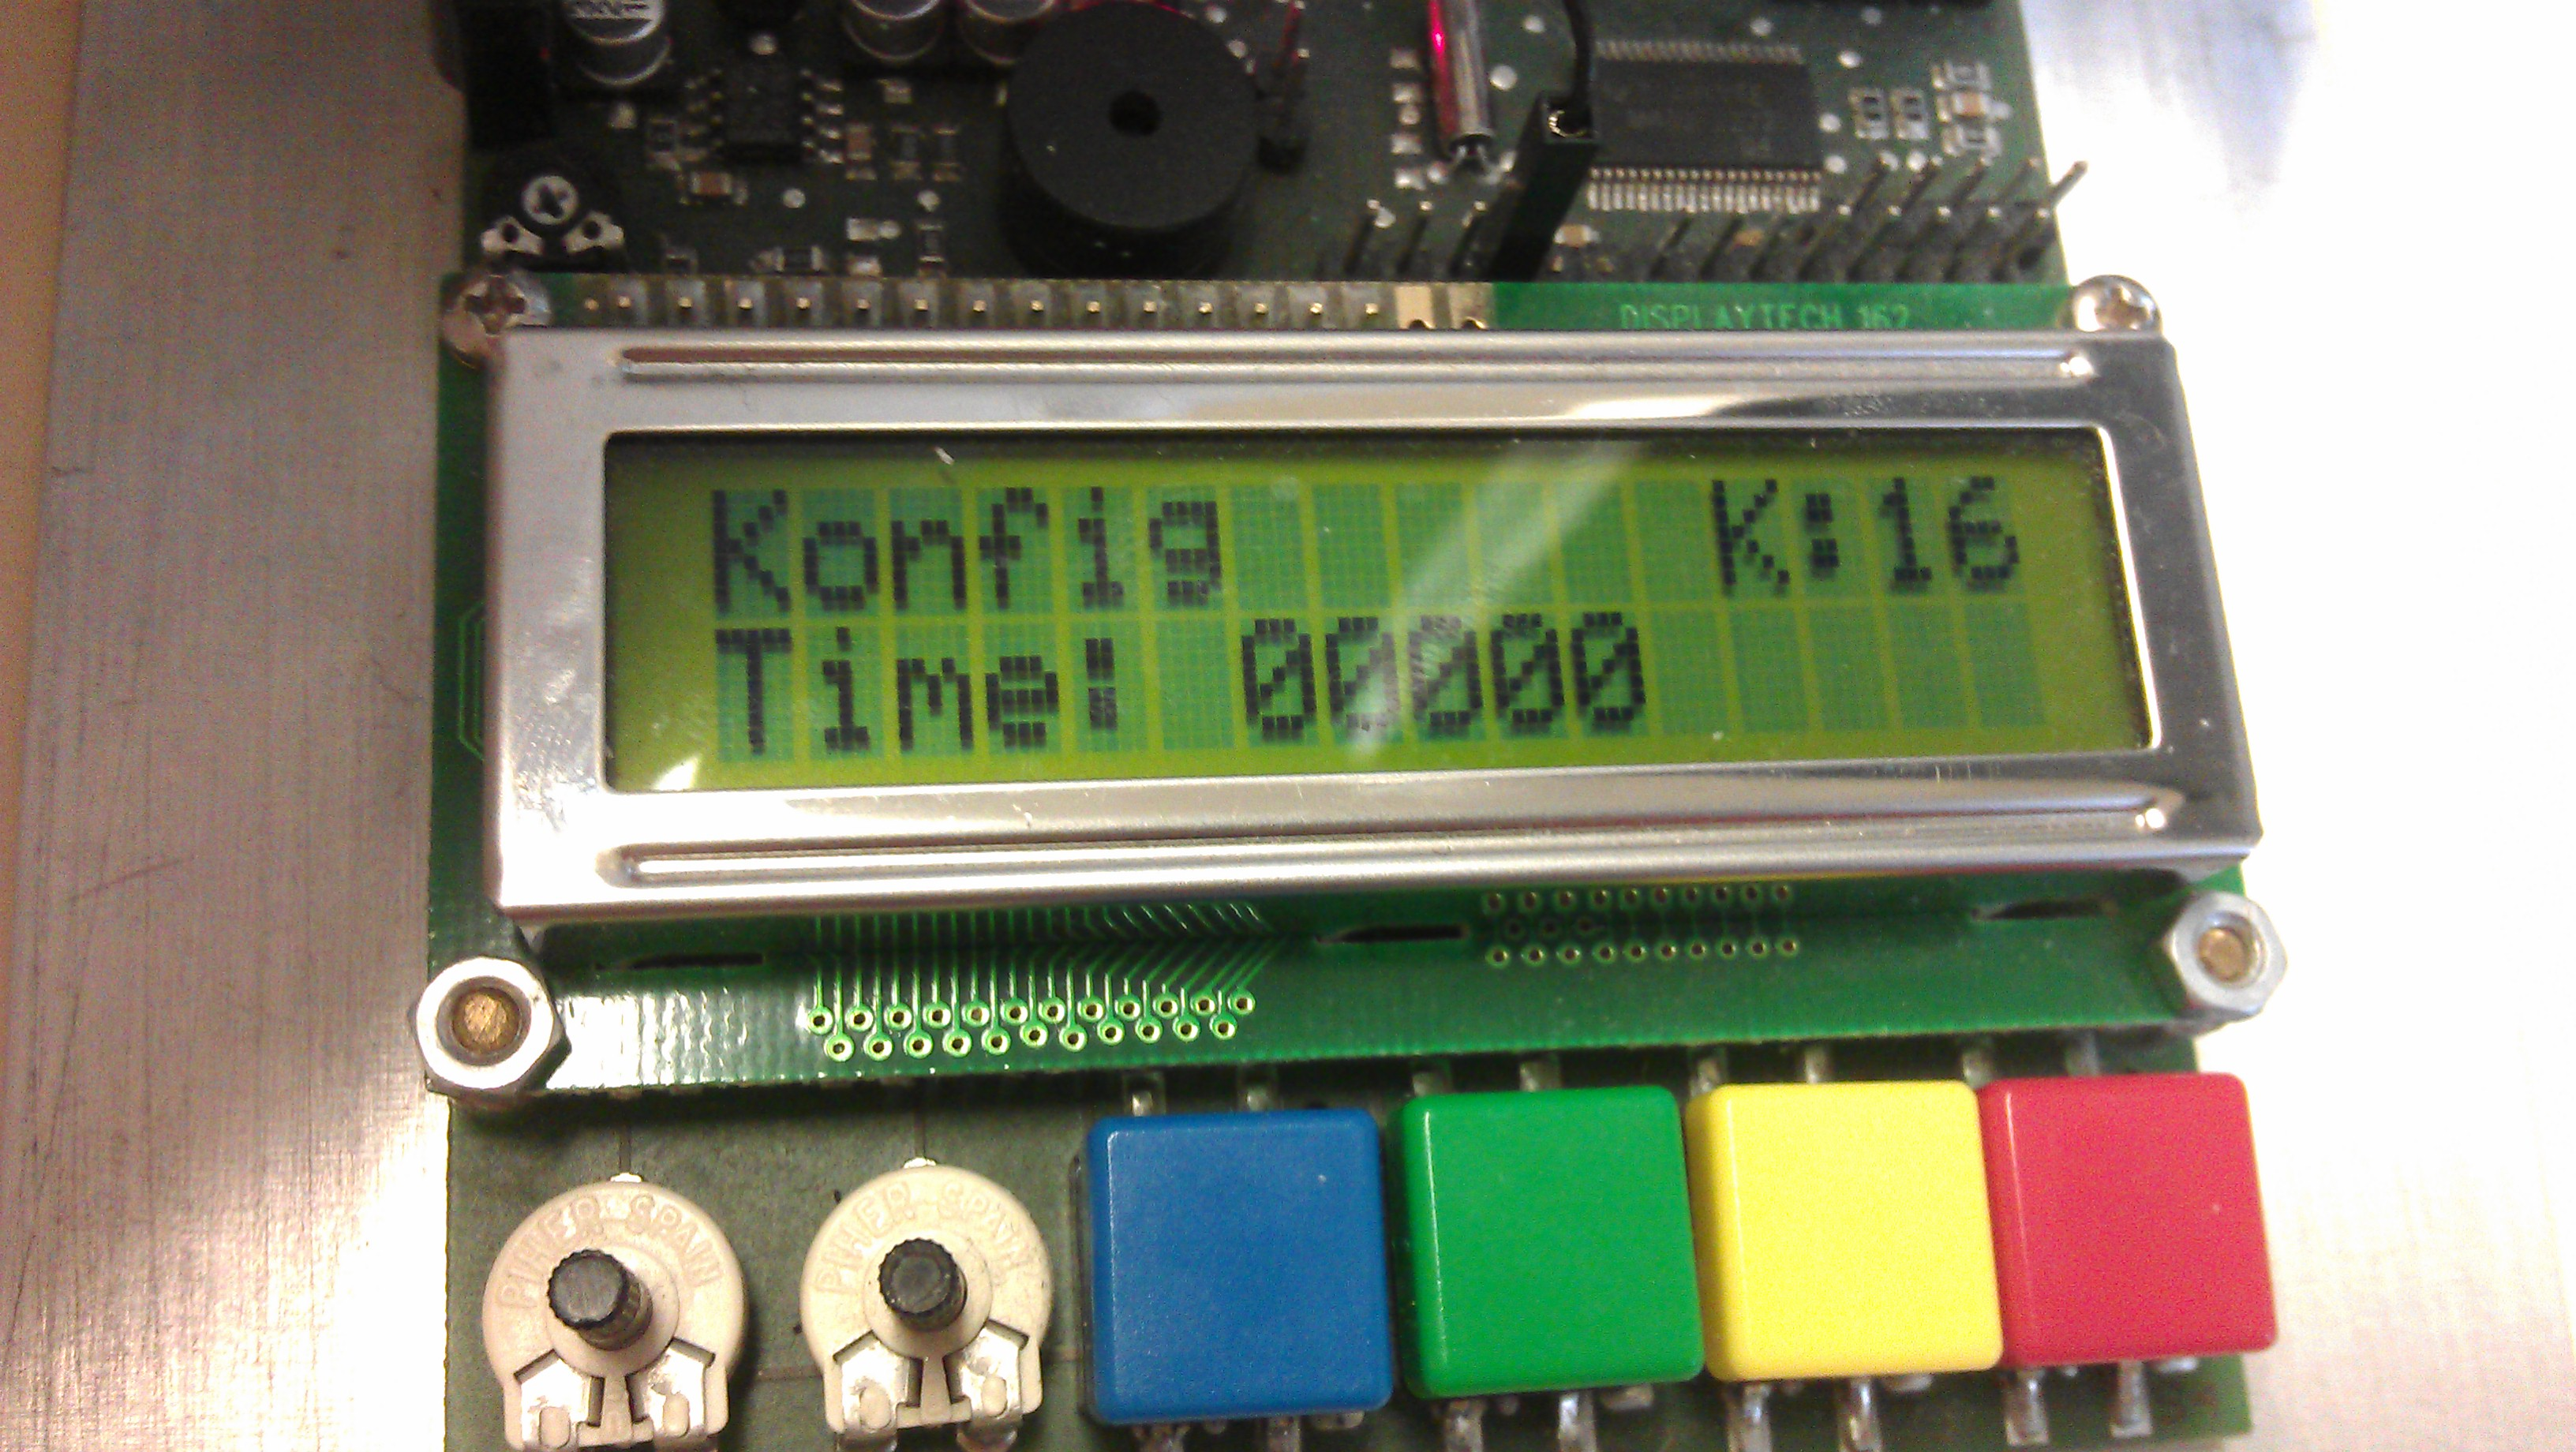
\includegraphics[width=0.7\linewidth]{img/Fernbedienung.jpg}
	\captionof{figure}{Teatimer im Konfigurationsmodus\newline links oben: Zustand, rechts oben: letztes Kommando, links unten: eingestellte Zeit}
	\label{fig:FernbedienungKonfig}
\end{minipage}

\vspace{1em}
Das vollständige Programm kann Anhang \ref{sec:Fernbedienung} entnommen werden.
 
\pagebreak



% ----------------------------------------------------------------------------------------------------------
% Interrupt-Technik
% Die Analysen und Erklärungen zu den drei Programmen mit Interruptproblemen ----------------------------------------------------------------------------------------------------------
\section{Analyse praktischer Probleme mit Interrupts}
In der nachfolgenden Diskussion wird, durch die Analyse dreier Programme, auf häufig auftretende und in der Praxis zu beachtenden Tücken im Umgang mit der Interrupt-Technik aufmerksam gemacht.

\subsection{Praktikumsaufgabe 22 - Interrupt-gesteuertes Programm I}
Der Timer wurde mit unterschiedlichen Capture-/Compare-Werten konfiguriert (TACCR0-Register). Anschließend wurde jeweils die benötigte Zeit gemessen, um 1000 Interrupts zu erzeugen. Es wurde erwartet, dass bei einem doppelt so hohen Capture-/Compare-Wert es genau doppelt so lange dauert, bis die 1000 Interrupts erreicht sind, also eine Proportionalität besteht.

\begin{table}[!htb]
	\centering
	\begin{tabular}{@{}c|c@{}}
		\toprule
		CCR0-Wert & Zeit für 1000 Interrupts in ms \\ \midrule
		200       & 16,2                           \\
		150       & 10,5                           \\
		100       & 9,4                            \\
		50        & 9,4                            \\ \bottomrule
	\end{tabular}
	\caption{Messergebnisse}
\end{table}

Die Messungen ergaben, dass die höhere Werte ansatzweise proportional zu der benötigten Zeit sind. Bei kleineren Werten, hier 100 und 50, konnte allerdings kein Unterschied in der benötigten Zeit festgestellt werden. Außerdem wurde der Ausgabestring \glqq aktuell \grqq{} bei diesen Werten nicht vollständig auf dem Display dargestellt.

Daraus wurde geschlussfolgert, dass die ISR durch die beinhaltenden LCD-Operationen länger dauert als die Zeitdauer zwischen dem Auftreten der einzelnen Interrupts, wenn der Zählwert zu deren Auslösung zu klein gewählt ist. Einfacher formuliert, die Interrupts werden durch den niedrigen Zählwert so schnell ausgelöst, dass der vorherige Interrupt noch nicht abgearbeitet werden konnte. Dieses Verhalten lässt sich ungefähr bis zu einem Zählwert von 100 bis 150 beobachten. Darüber hinaus werden vorherige ISRs vor dem Eintreffen des nächsten Interrupts vollständig durchgeführt.


Es gibt mehrere Ansätze diesem Sachverhalt zu begegnen:
\begin{description}
	\item[1. Lösungsvorschlag:] Unter der Prämisse, dass die langwierigen LCD-Operationen in der ISR stehenbleiben, könnte man diese nur alle x-Aufrufe ausführen. Das Display wird demnach intervallartig aktualisiert.
	
	\textbf{Pro:} regelmäßge Darstellung des aktuellen Wertes auf dem Display, auch bei kleinen CC0-Zählwerten.
	
	\textbf{Contra:} verfälscht das Messergebnis leicht. 
	
	\item[2. Lösungsvorschlag:] In der ISR wird lediglich die Zähler-Variable inkrementiert. Die LCD-Operationen werden in die Endlosschleife innerhalb der main-Funktion verschoben, damit die einzelnen ISRs schneller abgearbeitet werden können.
	
	\textbf{Pro:} verfälscht das Messergebnis nicht.
	
	\textbf{Contra:} nur bei größeren Zählwerten möglich, da bei kleinen keine Zeit zwischen den ISR-Aufrufen vorhanden ist um in die main-Funktion zurückzukehren. Auf eine ISR folgt direkt die Nächste.
\end{description}

\subsection{Praktikumsaufgabe 23 - Interrupt-gesteuertes Programm II}
Während der Analyse des Programms wurde beobachtet, dass die LEDs und das LCD-Display einen unterschiedlichen Wert anzeigen, obwohl sie nacheinander über die gleiche Variable beschrieben werden. Diese Variable \glqq Zaehler\grqq{} wird jedes mal in der zugehörigen ISR inkrementiert, wenn ein Interrupt von Port 2 ausgelöst wird. Am Ende dieser ISR wechselt ein Flag namens \glqq Zaehlerveraendert\grqq{} auf TRUE. Infolge dessen wird in der Endlosschleife die Aktualisierung erst des LCDs, dann der LEDs vorgenommen. 

Das Problem bei dieser Art von Programmierung ist, dass nicht bedacht wurde, dass zwischen diesen beiden Aktualisierungen ein erneuter Interrupt ausgelöst werden kann, der die Variable \glqq Zaehler\grqq{} verändert. 
Das Resultat ist, dass die LEDs mit einem anderen Wert beschrieben werden, als es zuvor das LCD wurde, wodurch die Darstellung inkonsistent ist. 

Diese Problematik ist als Shared-Data-Bug bekannt. Ein Ansatz diesem in dieser Situation zu begegnen, ist es eine Hilfsvariable anzulegen, die am Anfang der Endlosschleife mit dem Wert von \glqq Zaehler\grqq{} beschrieben wird. Anschließend wird diese Variable zur Aktualisierung der beiden Anzeigegeräte verwendet, wodurch sich zwischenzeitliche Interrupts nicht bemerkbar machen. Die Wertzuweisung an die Hilfsvariable kann ebenfalls nicht von einem Interrupt unterbrochen werden, da diese vom Typ Character wäre und somit innerhalb eines Taktes mithilfe eines Maschinenbefehls vonstatten ginge.


\subsection{Praktikumsaufgabe 24 - Interrupt-gesteuertes Programm III}
Während der Analyse des Programms wurde beobachtet, dass die zweite If-Bedingung der Endlosschleife nach einer gewissen Zeit erfüllt und somit der Text \glqq Seltsam, oder?!\grqq{} auf das LCD-Display ausgegeben wurde. Dies dürfte eigentlich nie passieren, da die Bedingung so konstruiert ist, dass sie durch den bestehenden Code nicht erfüllt werden kann.

Das Problem ist hier der Datentyp Long in Verbindung mit der Interrupt-Technik.
Der MSP430 ist ein 16-Bit-Prozessor. Dies hat zur Folge, dass ein Integer-Typ typischerweise 16 Bit und ein Long-Typ 32 Bit groß ist. Wenn eine Variable eines solchen Typs bspw. einen Wert zugewiesen bekommt, sind zwei Maschinenbefehle die Folge. Der eine überträgt das Low-Word und der andere das High-Word, denn die Variable muss auf zwei 16-Bit Speicherplätze verteilt werden.

Zur Veranschaulichung der Problematik betrachte man untenstehenden Assemblercode, der aus diesem C-Code hervorgeht:

\begin{lstlisting}[caption=C-Code MSP430, label=lst:LongInterruptC]
if ( (Zaehler > (oldZaehler+100) ) || (Zaehler < (oldZaehler-100) ) ) {...}
\end{lstlisting}

Der Wert von OldZaehler wird in Register 14 und 15 der CPU geladen. Zuerst das Low-Word (0x204) und dann das High-Word (0x206).
\begin{lstlisting}[caption=Assemblercode MSP430, label=lst:LongInterruptA1]
008070   421E 0204     mov.w   //&oldZaehler,R14
008074   421F 0206     mov.w   //&0x206,R15
\end{lstlisting}

Auf das Low-Word wird nun die Dezimalzahl 100 (0x64) addiert und das Carry-Bit (Übertrag) auf das High-Word geschrieben, womit dessen vorheriger Inhalt hinfällig ist.
\begin{lstlisting}[caption=Assemblercode MSP430, label=lst:LongInterruptA2]
008078   503E 0064     add.w   //0x64,R14
00807C   630F          adc.w   //R15
\end{lstlisting}

Danach werden die Werte in zwei Stufen verglichen, gegebenfalls gesprungen und ein äquivalentes Prozedere mit dem zweiten Teil der If-Anweisung durchgeführt:
\begin{lstlisting}[caption=Assemblercode MSP430, label=lst:LongInterruptA3]
00807E   912F 0202     cmp.w   //&0x202,R15
008082   3812          jl      //0x80A8
008084   2003          jne     //0x808C
008086   921E 0200     cmp.w   //&Zaehler,R14
00808A   280E          jnc     //0x80A8

00808C   421E 0204     mov.w   //&oldZaehler,R14  
008090   421F 0206     mov.w   //&0x206,R15
008094   503E FF9C     add.w   //#0xFF9C,R14
008098   633F          addc.w  //#0xFFFF,R15 
00809A   9F82 0202     cmp.w   //R15,&0x202
00809E   3804          jl      //0x80A8
0080A0   23D8          jne     //0x8052
0080A2   9E82 0200     cmp.w   //R14,&Zaehler
0080A6   2FD5          jc      //0x8052
\end{lstlisting}

Wird nun während des zweistufigen Vergleichs ein Interrupt ausgelöst und die Variable Zaehler durch die ISR inkrementiert, ist die If-Bedingung erfüllt.
\begin{description}
	\item[Lösungsansatz:] Dieses Problem lässt sich bei dem Datentyp Long nicht beheben. Man kann ihn lediglich versuchen so gut es geht zu vermeiden oder in solchen kritischen Abschnitten Interrupts kurzfristig abschalten. Zumindest in soweit, dass Variablen der kritischen Abschnitte nicht durch ISRs verändert werden, während man sich gerade in einem solchen Abschnitt befindet.
\end{description}
\pagebreak
% ----------------------------------------------------------------------------------------------------------
% Theoretische Praktikumsaufgaben
% Antworten auf die Frageblöcke der Praktikumsanleitung, woweit auch praktisch bearbeitet. ----------------------------------------------------------------------------------------------------------
\section{Theoretische Aufgabenstellungen}
Unter diesem Abschnitt sind die, zu bestimmten Aufgaben in der Praktikumsanleitung vorkommenden Frageblöcke, mit einer ausführlichen Antwort versehen worden.

\subsection{Block 1 - Erste Schritte / IDE}
\paragraph{Was ist ein Crosscompiler?}
Ein Crosscompiler erzeugt beim Übersetzungsvorgang einen Zielcode der für eine andere Prozessorarchitektur als die Eigene ausgelegt ist. Bei uns ist dieser Teil der IAR-Entwicklungsumgebung und erzeugt Zielcode für den MSP430, anstatt für den in der Workstation verbauten Prozessor.
\paragraph{Was ist eine JTAG-Schnittstelle?}
Eine JTAG-Schnittstelle wird unter anderem für die Übertragung des Maschinencodes vom Entwicklungsrechner zum Education Board benutzt. Des Weiteren kann mit ihr die Programmausführung gesteuert werden, was bedeutet das In-System-Debugging möglich ist.

\subsection{Block 2 - Erste Schritte / Blinkprogramm }
\paragraph{Warum kann der Parameter Anzahl in der Funktion Warteschleife nicht vom Typ int sein?}
Bei unserem MSP430 handelt es sich um ein 16-Bit-Prozessorsystem, wo ein Integer typischerweise dann auch 2 Byte groß ist. Ein signed Integer hat also einen Datenbereich von -32.768 bis 32.767. Die ursprüngliche Schleife war auf einen Wert von 50.000 notiert, weswegen ein Überlauf stattgefunden hätte. Das führt letztlich dazu, dass die Laufbedingung der For-Schleife i\textgreater0 nicht zutrifft, die Schleife nie läuft und somit die  Warteschleife nichtig wird.
\paragraph{Welche Hardwaregruppen werden angesprochen?}
Das Kontrollregister des Watch-Dog-Timers WDTCTL, das Richtungsregister P1DIR und das Ausgangspufferregister P1OUT werden angesprochen.
\paragraph{Warum muss man keine Hardwareadressen angeben um die Hardware anzusprechen?}
In der inkludierten Headerdatei msp430x22x2.h sind für die Hardwareadressen symbolische Namen, mittels Makrodefinitionen, angelegt.
\paragraph{Wie ist die Hardwareadresse von P1OUT? Wie kann man das herausfinden?}
Die Hardwareadresse von P1OUT ist 0x0021. Diese Information kann man entweder in der Headerdatei msp430x22x2.h oder unter der Rubrik 8.3 Digital I/O Resgisters im Family Users Guide (S.333) des Mikrocontrollers nachlesen. 
\paragraph{Warum wird der Watchdog Timer ausgeschaltet?}
Der Watch-Dog-Timer ist standardmäßig eingeschaltet und hat die Aufgabe ein Versagen des Systems durch Softwarefehler zu vermeiden. Die Software muss typischerweise dem Watch-Dog-Timer in regelmäßigen Abständen mitteilen, dass sie sich noch in einem konsistenten Zustand befindet. Erfolgt dies nicht, setzt der Watchdog das Gerät automatisch in einen definierten Ausgangszustand zurück. Da wir in der ersten Praktikumsaufgabe LED-Lauflicht softwaretechnisch eine Endlosschleife  umgesetzt haben musste dieser einerseits zuvor ausgeschaltet werden. Andererseits handelt es sich bei unseren Praktikumsaufgaben nicht um kritische Anwendungen, wo ein aktiver Watch-Dog-Timer vonnöten wäre.
\paragraph{Wie funktioniert In-System-Debugging?}
Nach der Übersetzung des C-Programmes wird dieses über die JTAG-Schnittstelle in den Flash-Speicher des Mikrocontrollers geladen. Anschließend wird es zur Ausführung gebracht. Dabei stehen zusätzlich verschiedene Debug-Möglichkeiten wie das setzen von Breakpoints, Inspektion der Speicherplätze und Register, Stepping, Tracing usw. zur Verfügung. Das Debugging erfolgt echt auf dem Chip, sodass die Befehle direkt von der Hardware umgesetzt werden. Dazu wird eine spezielle Kontrollhardware benötigt, die die Kontrolle über den Programmlauf behält und Kommandos und Informationen über die JTAG-Schnittstelle mit der IDE synchronisiert.

\subsection{Block 3 - Interrupt über Port 2}
\paragraph{Was bedeutet die Zeile "\#pragma vector=PORT2\_Vector"?}
Dieser Funktionsvorsatz ist eine Anweisung an den Compiler, die Adresse dieser Funktion an die Stelle die für Port 2 in der Interrupt-Vektoren-Tabelle vorgesehen ist, einzutragen. Wenn nachfolgend ein Interrupt von Port 2 ausgelöst wird, wird dort über die hinterlegte Adresse genau diese Funktion (ISR) aufgerufen und ausgeführt.

\paragraph{Warum wird hier vor den Funktionsnamen "\_\_interrupt" gesetzt?}
Es handelt sich um einen ergänzenden Typbezeichner. Dieser weist den Compiler an, die damit versehene Funktion als Interrupt-Service-Routine zu übersetzen, also speziellen Programmcode zusätzlich zu erzeugen. Dieser sorgt insbesondere dafür, dass alle Register und Flags vor dem Aufruf auf dem Stack durch \textit{push}-Befehle gesichert und nach dem Aufruf zurückgeschrieben werden, damit unter anderem an die vorherige Stelle im Programmcode zurückgesprungen werden kann und die zuvor benutzen Register und Flags auch die zu erwartenden Werte aufweisen. Das Statusregister im Besonderen wird durch den \textit{reti}-Befehl am Ende der Funktion zurückgeschrieben.

\paragraph{Warum können keine weiteren Interrupts eintreten, wenn man in der Interrupt-Service-Routine ist?}
Durch die Voreinstellung des Chips wird bei Eintreten in eine Interrupt-Service-Routine das Statusregister vollständig gelöscht. Dadurch wird auch das GIE-Bit (Global Interrupt Enable) auf 0 gesetzt. Somit können keine weiteren Interrupts bis zum Wiederherstellen des Statusregisters beim Beenden der ISR eintreten. Allerdings kann eine Prioritätenregelung aktiviert werden, um höher priorisierte Interrupts das Unterbrechen von Interrupt-Service-Routinen niedrigerer Priorität zu ermöglichen. \cite[Seite 38]{MSP430x2xx.Users.Guide}


\subsection{Block 4 - Zyklische Interrupts durch den Timer}
\paragraph{Warum läuft der Timer A nach dem Befehl "TACTL = TASSEL0 + TACLR;" noch nicht gleich?}
Der Befehl bewirkt lediglich, dass das Controlregister des Timers A als Eingangstakt TAClock zugeführt und das Zählregister auf 0 zurückgesetzt wird. Der Timer befindet sich allerdings noch im Stop-Mode. Über die Mode-Control-Bits kann dieser in verschiedenen Modi gestartet werden. Dies wird erreicht, in dem bspw. die Makrodefinition MC\_1 - MC\_3 gleich mit verodert werden (TACTL = TASSEL0 + TACLR + MC\_1), um den Timer direkt starten zu lassen oder dem Anwendungszweck entsprechend, erst später (TACTL \text{\textbar}= MC\_1). 

\paragraph{Welche Signale kann man dem Eingang des Timers (außer AClock) zuführen?} Als interne Taktquelle kann außer der AClock die SMClock verwendet werden. Als externe Taktquellen können TAClock und INClock zugeführt werden.

\paragraph{Wie funktioniert der Up Mode des Timers A und welche Modes gibt es noch?} Im Up-Mode zählt der Timer aufwärts, bis er den zuvor spezifizierten Wert im Capture-/Compare-Register erreicht. Beim nächsten Takt beginnt er erneut von 0x0000 zum angeben Wert hochzuzählen. Dieser kann maximal 0xFFFF sein, welches äquivalent zum Continuous-Mode wäre. Den Up-Mode kann man als Zählbetrieb des Timers bezeichnen, bei dem von außen kommende Impulse mithilfe der Interrupt-Technik gezählt werden können. Wenn diese eingeschaltet werden, wird jedes mal bei Erreichen des Zählwertes vor dem Umschalten auf 0x0000 ein Interrupt ausgelöst. Zu den bereits genannten Stop-, Up- und Continuous-Mode gibt es noch den Up/Down-Mode, in dem bei Erreichen des Caputre-/Compare-Wertes von diesem an bis 0x0000 runtergezählt wird und anschließend wieder hoch, anstatt wie beim Up-Mode direkt auf 0x0000 zu wechseln.

\paragraph{Mit welcher Taktfrequenz läuft unser Edu-Board?}
Das Edu-Board läuft mit dem Takt, mit dem die CPU betrieben wird. Dieser liegt zwischen 12 kHz und 16 MHz. \cite[Seite 6]{MPT.Praktikum.Wuest}


\subsection{Block 5 - Impulse von rotierender Welle zählen und anzeigen}
\paragraph{Aus welcher Quelle sollten die Impulse am Zählereingang kommen?}
Sie sollten von TAClock bzw. TBClock kommen, je nachdem welchen Timer man zum Impulszählen benutzt.

\paragraph{Welchen Timer könnte man benutzen?}
Es kann sowohl Timer A als auch Timer B benutzt werden. Es sollte allerdings beachtet werden, dass Timer A ein festes 16-Bit-Zählregister hat, wohingegen man dieses bei Timer B softwaremäßig auf 8, 10, 12 oder eben 16 Bit einstellen kann. Weitere kleine Unterschiede können unter 13.1.1 Similarities and Differences From Timer\_A des Family Users Guide \cite{MSP430x2xx.Users.Guide} nachgelesen werden. 

\paragraph{Welche Impulsquelle wird benutzt?}
Die rotierende Scheibe ist schwarz/weiß gestreift, wodurch es einer angebrachten Reflexlichtschranke möglich ist, bei Farbwechsel die Impulse auszulösen.

\paragraph{In welchem Mode sollte der Timer betrieben werden?}
 Da kein zu erreichender Zielwert existiert und kein Interrupt ausgelöst werden muss, ist der Continuous-Mode am besten für diese Aufgabe geeignet.

\paragraph{Wo nimmt man die nötigen Einstellungen vor?}
Sie werden im Controlregister des entsprechenden Timers vorgenommen. Bei Timer A wäre dies TACTL und bei Timer B TBCTL.

\paragraph{Wie oft sollte man die Anzeige aktualisieren?}
Es sollte ein Wert gewählt werden, der die langsamen LCD-Operationen berücksichtigt, damit keine Anzeigefehler auftreten. Da das Display lediglich vom menschlichen Auge abgelesen wird, reicht ein Intervall von einer halben bis einer Sekunde aus.

\paragraph{Kann bei Zählerbetrieb ein Low-Power-Mode genutzt werden, wenn ja, welche?} Es können die Low-Power-Modi 0 bis 3 genutzt werden. Der Low Power Mode 4 kann nicht zum Einsatz kommen, da dort auch alle Oszillatoren gestoppt werden, durch die der Timer versorgt wird.


\subsection{Block 6 - Anzeige der Drehzahl des rotierenden Rades}
\paragraph{Wie kann grundsätzlich eine Drehzahl gemessen werden?}
Die Drehzahl gibt die Anzahl der Umdrehungen N pro Zeitintervall T an, also wie häufig eine Umdrehung in dieser Zeit vollzogen werken konnte. Mathematisch ausgedrückt:
\[ n = \frac{\Delta N}{\Delta T}  \]
In unserem Fall der Reflexlichtschranke macht es Sinn, die Impulse pro Sekunde zu messen, zu ermitteln, wie viele Impulse eine vollständige Umdrehung ausmachen und die Drehzahl in der Einheit Umdrehungen pro Minute auszugeben. 

Achtung Praxis: Überläufe des Zählregisters beachten und vorzugsweise mit gekürzten Werten rechnen.

\paragraph{Wie viele Timer braucht man?}
Man braucht 2 Timer. Der eine misst die Impulse, welche zur Berechnung der Umdrehungsanzahl benötigt werden (im Continuous-Mode). Der andere gibt das Zeitintervall an, indem die Drehzahlberechnung zyklisch stattfindet. Dazu wird der Up-Mode benutzt, das Capture-/Compare-Register mit einem entsprechenden Wert belegt, Interrupts eingeschaltet und bei jeder Auslösung eines solchen die Drehzahlberechnung durchgeführt. 


\subsection{Block 7 - Analoges Signal von Potentiometern anzeigen}
\paragraph{Wozu werden die beiden internen ADC-Kanäle genutzt?}
Sie werden für den internen Temperatur-Sensor und zur Größenermittlung der externen Referenzspannung genutzt.

\paragraph{Welche Konvertierungsarten (Conversion Modes) kennt der ADC10?}
Es gibt vier Konvertierungsarten:
\begin{itemize}
	\item single channel single-conversion
	\item sequence-of-channels
	\item repeat single channel
	\item repeat sequence-of-channels
\end{itemize}

\subsection{Block 8 - Interrupt über Port 2 unter Berücksichtigung energieeffizenter Programmierung}
\paragraph{Bei Eintritt eines Interrupts beendet der MSP430 automatisch den Low-Power-Mode und wechselt in den Active-Mode, Warum ist das sinnvoll und wie wird es technisch durchgeführt?} Diese Vorgehen ist nicht nur sinnvoll, sondern auch notwendig, weil der CPU-Takt unterbrochen wurde und somit keine Maschinenbefehle ausgeführt werden können, um Low-Power-Mode manuell zu beenden.
Technisch umgesetzt wird dies über das Statusregister der CPU. In diesem kann das Bit CPUOFF gesetzt (1: CPU inaktiv) und gelöscht werden (0: CPU aktiv). Standardmäßig steht dieses auf 0. Wird die CPU verleitet in einen Low-Power-Mode zu schalten, wird das Bit auf 1 gesetzt. Kommt während sich die CPU im Low-Power-Mode befindet ein Interrupt, wird dieses Bit gelöscht, die ISR abgearbeitet und danach das Bit erneut gesetzt, wodurch das System zurück in den Low-Power-Mode versetzt wird.

\paragraph{Welche Low-Power-Modes sind bei dem oben stehenden Programm möglich?} Alle Low-Power-Modes (0 bis 4) sind möglich, da Interrupts nicht durch diese abgeschaltet werden.

\paragraph{Welche Low-Power-Modes sind möglich beim Taschenrechner?} Alle Low-Power-Modes (0 bis 4) sind möglich.

\paragraph{Welche Low-Power-Modes sind möglich beim Tea-Timer?}
Es können die Low-Power-Modi 0 bis 3 genutzt werden. Der Low Power Mode 4 kann nicht zum Einsatz kommen, da dort auch alle Oszillatoren gestoppt werden, durch die der Timer versorgt wird. Die Zeit könnte nicht mehr runtergezählt werden.

\paragraph{Kann man an unserem Education System das Absinken des Versorgungsstromes beim Eintritt in einen Low-Power-Mode messen?} Ja, kann man. Die Leistungsaufnahme reduziert sich, dies ist messbar. 

\pagebreak
% ----------------------------------------------------------------------------------------------------------
% Die Bearbeitung der Aufgaben 13.6 und 13.7 (Verständnis von Maschinencode) sowie 12.1 und 12.2 (Memory-Map in der Endfassung mit Variableneintragung) aus dem MPT-Skript.
% ----------------------------------------------------------------------------------------------------------
\section{Aufgabenstellungen des MPT-Skripts}
Im Folgenden werden die Aufgaben 12.1, 12.2 (Memory Map), 13.6 und 13.7 (Aufgaben zum Verständnis von Maschinencode) aus dem MPT-Skript besprochen.

\subsection{Memory Map}
Der Speicher des MSP430F2274 wird nachfolgend in Form einer Landkarte dargestellt. Hierbei wird zunächst auf den prozessoreigenen Speicher eingegangen und im Anschluss auf die Aufteilung des Hauptspeichers in seine funktional unterschiedlichen Bereiche.

\vspace{1em}
\begin{minipage}{\linewidth}
	\centering
	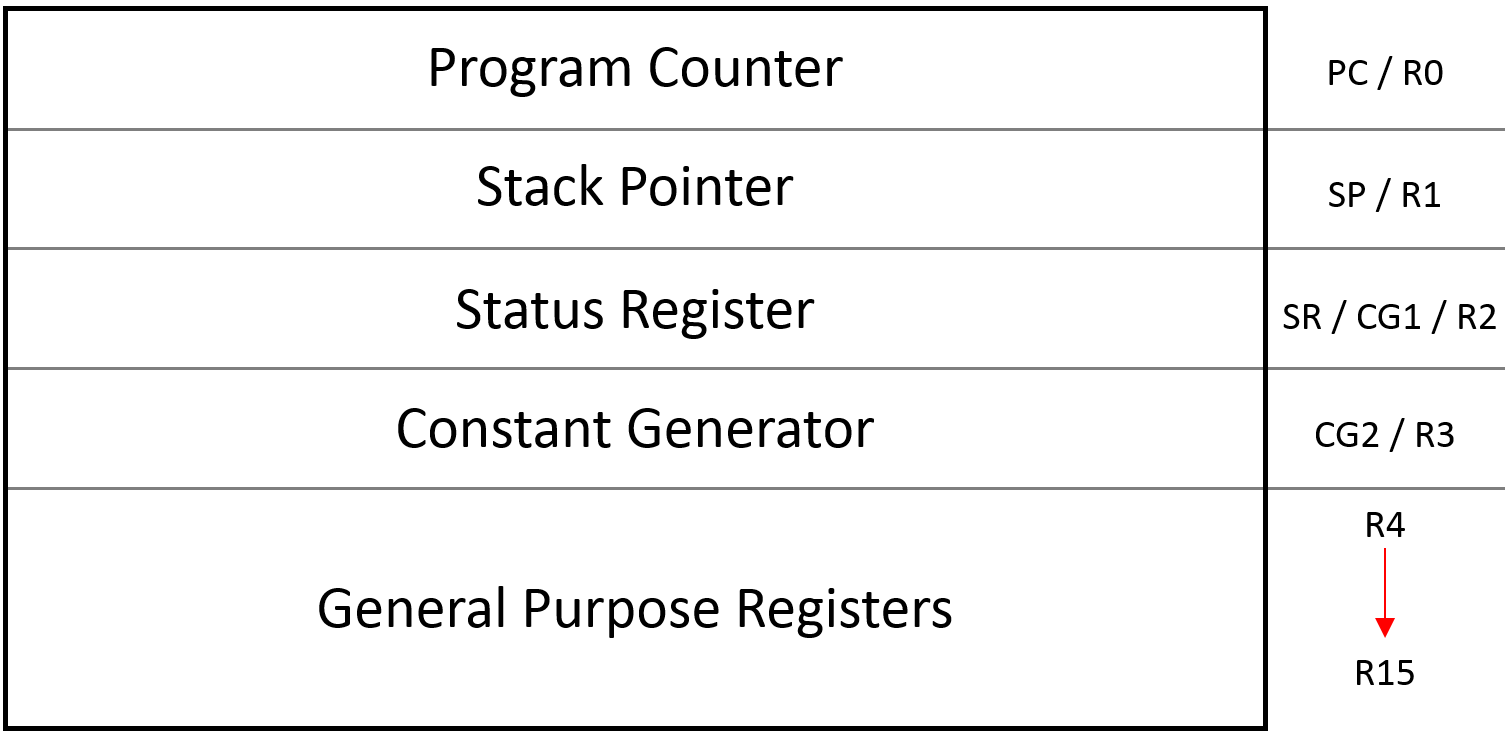
\includegraphics[width=0.7\linewidth]{img/MemoryMapCPU.png}
	\captionof{figure}[MemoryMapCPU]{Memory Map der CPU}
	\label{fig:MemoryMapCPU}
\end{minipage}
\vspace{0.5em}

Diese Abbildung illustriert den Registersatz der CPU. Insgesamt umfasst dieser 16 Register, wobei die ersten vier eine oder mehrere Spezialrollen einnehmen können.

\vspace{1em}
\begin{minipage}{\linewidth}
	\centering
	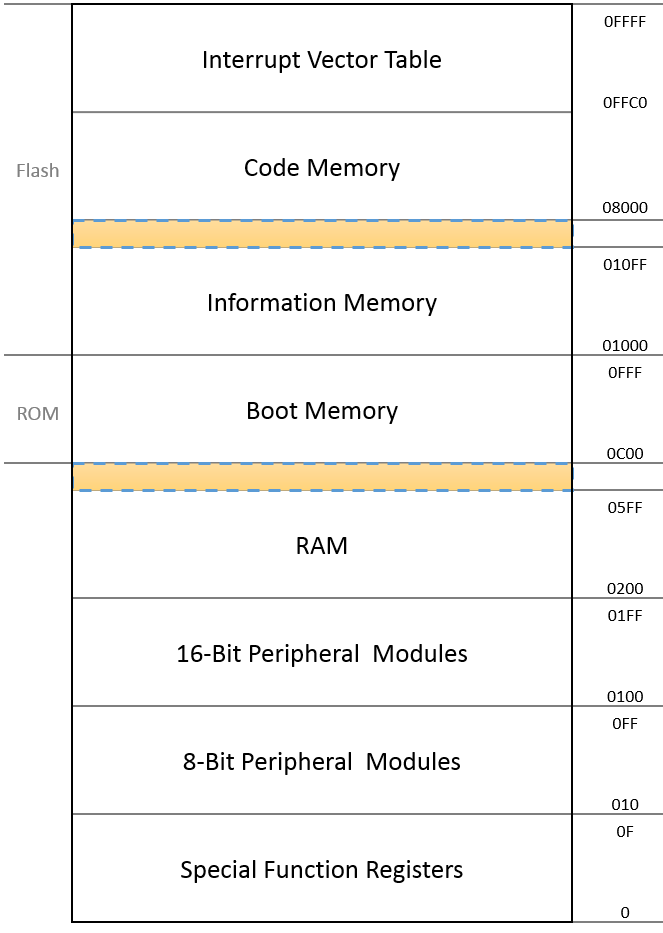
\includegraphics[width=0.7\linewidth]{img/MemoryMapSpeicher.png}
	\captionof{figure}[MemoryMapSpeicher]{Memory Map des Hauptspeichers}
	\label{fig:MemoryMapSpeicher}
\end{minipage}
\vspace{0.5em}

Obige Abbildung zeigt die Aufteilung des Hauptspeichers in die funktional unterschiedlichen Bereiche. Von diesen sind zusätzlich Anfangs- und Endadressen in hexadezimaler Schreibweise vermerkt. Die ersten drei Bereiche bilden zusammen den Flash-Speicher sowie das Boot Memory das ROM. Die beiden farblich abgehobenen Sektionen bilden bei dem MSP430F2274 nicht adressierbare Speicherbereiche ab.

\vspace{1em}
\begin{minipage}{\linewidth}
	\centering
	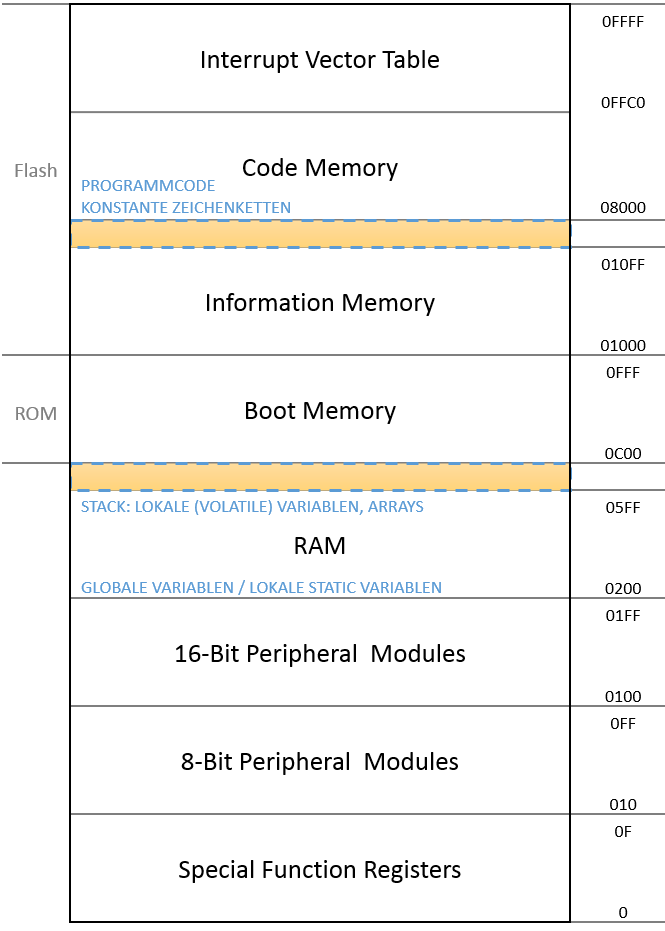
\includegraphics[width=0.7\linewidth]{img/MemoryMapSpeicherProg.png}
	\captionof{figure}[MemoryMapSpeicherProg]{Memory Map des Hauptspeichers mit Kennzeichnung der Programmcode-Elemente}
	\label{fig:MemoryMapSpeicherProg}
\end{minipage}
\vspace{0.5em}

In dieser erweiterten Darstellung der Memory Map wurde kenntlich gemacht, wo Programmvariablen und sonstige Komponenten im Speicher während des Programmlaufes liegen. 

Der Stack beispielsweise befindet sich am oberen Ende des Adressbereichs des RAMs und wächst nach unten, wohingegen sich die Globalen und lokalen statischen Variablen an dessen unteren Ende befinden.

Die konkreten Speicherplätze der Programmteile des referierten Übungsprogramms sind in folgender Tabelle aufgelistet:

\begin{table}[]
	\centering
	
	\label{my-label}
	\begin{tabular}{|c|c|}
		\hline
		\textbf{    Programmteil     }                                       & \textbf{Speicherposition}                                         \\ \hline
		Programmcode                                                & ab 0x800C aufwärts                                                \\ \hline
		Stack                                                       & ab 0x600 abwärts                                                     \\ \hline \hline
		\multicolumn{2}{|c|}{Globale Variablen}                                                                                         \\ \hline
		globalVar                                                   & 0x200                                                        \\ \hline \hline
		\multicolumn{2}{|c|}{Lokale Variablen}                                                                                          \\ \hline
		string1                                                     & R10                                                               \\ \hline
		i                                                           & R11                                                               \\ \hline
		j                                                           & R14                                                               \\ \hline \hline
		\multicolumn{2}{|c|}{Lokale static Variablen}                                                                                   \\ \hline
		k                                                           & 0x202                                                        \\ \hline
		\multicolumn{2}{|c|}{\begin{tabular}[c]{@{}c@{}}Lokale volatile Variablen\\ (zur Vollständigkeit selbst angelegt)\end{tabular}} \\ \hline
		p                                                           & auf Stack, Offset 0 vom SP                                        \\ \hline \hline
		\multicolumn{2}{|c|}{Arrays}                                                                                                    \\ \hline
		Zahlen                                                      & auf Stack, Offset 2 vom SP                                        \\ \hline \hline
		\multicolumn{2}{|c|}{Konstante Zeichenkette}                                                                                    \\ \hline
		"Hallo Welt!"                                               & vor dem Programmcode, 0x8000                                      \\ \hline
	\end{tabular}
	\caption{Speicherplatzbelegung zur Aufgabe 12.2}
\end{table}


\subsection{Verständnis von Maschinencode}
Bei diesen beiden Aufgaben wurde ein Programm erst für den MSP430F2272 und anschließend für den MSP430F449 compiliert. Zu dem entstandenen Assembler- und Maschinencode wurden Fragen beantwortet.
\subsubsection{Analyse des Assembler- und Maschinencodes}

\begin{enumerate}
	\item \textbf{In welche Assembler- bzw. Maschinenbefehle werden die Zuweisungen aus C übersetzt?}
	
	Zuweisungen werden in den \textit{Move}-Befehl übersetzt.
	
		\begin{figure}[!ht]
			\centering
			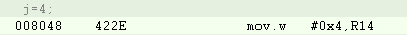
\includegraphics[width=0.7\textwidth]{img/MoveBefehl.png}
			\caption{eine Zuweisung}
		\end{figure}
	
	\item \textbf{In welche Assembler- bzw. Maschinenbefehle werden die Funktionsaufrufe aus C übersetzt?}
	
	Der \textit{call}-Befehl realisiert Funktionsaufrufe.
	
	\begin{figure}[!ht]
		\centering
		
\includegraphics[width=0.7\textwidth]{img/CallBefehl.png}
		\caption{der Funktionsaufruf von \textit{Warteschleife}}
	\end{figure}
	
	\item \textbf{Wie ist die Warteschleife auf Maschinenebene realisiert?}
	
	Zuerst wird mit \textit{tst.w} (hier genauer 0x930C) geprüft, ob der Wert in dem angegebenen Register (hier R12) 0 ist. Dieses Register beinhaltet die Laufvariable der For-Schleife. Die Statusbits werden abhängig von dem Ergebnis gesetzt und im nächsten Schritt durch ein \textit{jne} (Jump if not equal / Jump if Zeroflag not set) ausgewertet. Wenn das Zero-Bit nicht gesetzt ist, wird an die durch den Jump-Befehl angegebene Adresse gesprungen. Hier wird das Laufvariablen-Register durch die Addition von 0xFFFF um 1 dekrementiert. Anschließend erfolgt wieder das Testen durch \textit{tst.w}. 
		
	\begin{figure}[!htb]
		\centering
		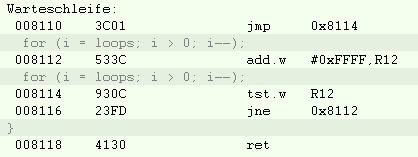
\includegraphics[width=0.7\textwidth]{img/Warteschleife.png}
		\caption{der Assembler- und Maschinencode zu \textit{Warteschleife}}
	\end{figure}
	\FloatBarrier

	
	Sollte durch das \textit{jne} nicht gesprungen werden (das letzte \textit{tst.w} setzte also das Zero-Bit im Statusregister), wird der nächste Maschinenbefehl ausgeführt: \textit{ret} - die Warteschleife-Funktion wird verlassen.
	
	\item \textbf{Wie wird der Mikrocontroller auf Maschinenebene in den Low-Power-Mode 3 umgeschaltet?}
	
	Dies wird mit dem Befehl \textit{bis.w} erreicht. \textit{Bis} steht für \glqq Set bits in destination\grqq. 
	
	\begin{figure}[!htb]
		\centering
		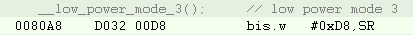
\includegraphics[width=0.7\textwidth]{img/LowPowerMode.png}
		\caption{das Setzen des Low-Power-Modes}
	\end{figure}
	
	Im Befehl ist die Adresse des Wortes, welches geändert werden soll, kodiert. Der direkt folgende Operand spezifiziert, welche Bits durch logisches Verodern auf 1 gesetzt werden sollen. Hier wird das Statusregister (R2) mit dem Wert 00D8 verodert.
	
	\begin{figure}[!ht]
		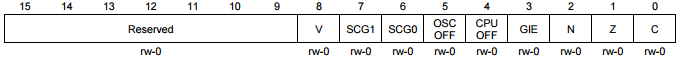
\includegraphics[width=1\textwidth]{img/Statusregister.png}
		\caption{Statusregister der MSP430x2xx-Family}
	\end{figure}
	\FloatBarrier
	
	Durch den \textit{bis}-Befehl werden SCG1, SCG2 und CPUOFF auf 1 gesetzt und somit die SMCLK, der DC0-Generator und die CPU ausgeschaltet. Dies entspricht der Konfiguration des Low-Power-Modes 3. Außerdem werden Interrupts global freigeschaltet (GIE - Bit 3). Dies ist nötig, da sonst der MSP ewig im Low-Power-Mode verweilen würde.
	
	\item \textbf{Was wird aus \_\_no\_operation(); auf der Assemblerebene und auf der Maschinenebene?}
	
	\_\_no\_operation() wird von dem Compiler in \textit{nop} übersetzt. Dieser Assemblerbefehl wird als \textit{MOV \#0, R3} (Maschinencode: 4303) emuliert. Das Register 3 ist ein Konstanten-Generator Register, welches nur als Quell-Register für Maschinenbefehle genutzt werden kann. Daher hat dieser Befehl keinen Effekt, beschäftigt also lediglich den CPU für einen Zyklus.
	%da müssen wir nochmal drüber gucken
	
	\item \label{Frage6}\textbf{Wo stehen die Operanden der Befehle ‘i=3’, ‘j=4’ und ‘k=5’ im Assembler- und im Maschinencode?}
	
	Eine Zuweisungen besteht aus zwei Operanden: dem Wert und die Adresse, wo dieser Wert abgespeichert werden soll.
	
	Die lokalen Variablen \textit{i} und \textit{j} werden in den Registern 11 und 14 gespeichert und können damit im Maschinencode direkt adressiert werden. Bei \textit{k} handelt es sich jedoch um eine statische Variable, welche daher im RAM abgespeichert wird. Der Adressraum des RAMs beginnt bei 0200h, k wird an der Adresse 0202h abgespeichert. Dies wird dem Maschinenbefehl als zusätzlicher Operand angehängt.
	
	\begin{figure}[!ht]
		\centering
		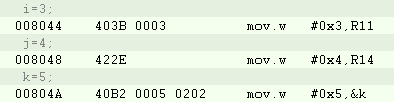
\includegraphics[width=0.7\textwidth]{img/Zuweisungen.png}
		\caption{verschiedene Varianten der Zuweisungen}
	\end{figure}
	
	Bei der Zuweisung \textit{i=3} wird der Zuweisungswert als erster Operand angegeben: 0003. Die 4 bei \textit{j=4} wird durch einen Konstanten-Generator erzeugt, welcher durch den Move-Befehl angesteuert wird: der Maschinencode 422E lautet in binär 0100 0010 0010 1110. Die ersten 4 Bit kodieren den Move-Befehl. Die zweiten 4 Bit definieren R2 als Quell-Register, die letzten 4 Bit R14 als Ziel-Register. Bei R2 handelt es sich um den Konstanten-Generator. Wird dieser mit der As-Konfiguration 10b (Bits 4 \& 5) angesprochen, liefert er eine 4.
	Eine 5 kann nicht durch einen Konstanten-Generator erzeugt werden, daher wird diese bei der Zuweisung \textit{k=5} ebenfalls als direkter Operand angegeben.
	
	\item \textbf{Können Sie erkennen, wo im Maschinencode die Nummer des angesprochenen Registers steht?}
	
	Siehe \ref{Frage6}.
	
	\item \textbf{Mit welchem Maschinenbefehl wird die Multiplikation \glqq\(k=i*j\)\grqq{} ausgeführt?}
	
	Für die Multiplikation wird eine spezielle Multiplikationsfunktion namens Mul16 durch einen \textit{call}-Befehl aufgerufen.
	
	
	\vspace{1em}
	\begin{minipage}{\linewidth}
		\centering
		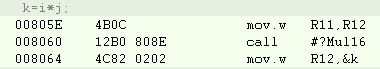
\includegraphics[width=0.7\linewidth]{img/MultF2274.png}
		\captionof{figure}[Multiplikation im Assemblercodes des MSP430F2274]{Multiplikation im Assemblercodes des MSP430F2274 }
		\label{fig:MultF2274}
	\end{minipage}
	
	
	\item \textbf{Wie wird die Multiplikation \glqq summe*9 \grqq{} in der Funktion \glqq rechne\grqq{} ausgeführt?}
	
	Eine Kopie des Wertes von \textit{summe} wird durch den Befehl \textit{rla} dreimal nach links rotiert. Dies entspricht einer dreimaligen Multiplikation mit 2. Anschließend wird der ursprüngliche Wert von summe dazu addiert. Dieser Vorgang lässt sich also mit folgender Rechnung zusammenfassen: \(summe*2*2*2+summe\). Dies ergibt \(summe*9\).
	
	\begin{figure}[!ht]
		\centering
		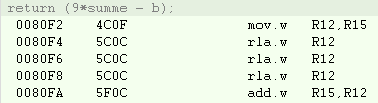
\includegraphics[width=0.7\textwidth]{img/Summe.png}
		\caption{\(summe*9\) im Assembler- und Maschinencode}
	\end{figure}
	
\end{enumerate}

\subsubsection{Codeerzeugung bei geänderter Hardwareplattform}

Im MSP430F449 ist der Speicher anders organisiert. Während beim MSP430F2274 die statischen Variablen und der Programmcode ab der Adresse 0800h des Flash-Speichers gespeichert wird, beginnt der selbe logische Speicherbereich beim MSP430F449 bei der Adresse 01100h des Speichers. Dadurch ändern sich natürlich alle Maschinenbefehle, die auf eine Adresse des statischen Speichers verweisen, wie \textit{call}, \textit{jump} und Befehle, welche mit statischen Variablen arbeiten.

Des weiteren werden die Register in einer anderen Reihenfolge mit den nicht-statischen lokalen Variablen belegt. Die statischen lokalen Variablen werden bei beiden Hardwareplattformen im RAM mit identischer Basisadresse gespeichert. Eine Übersicht über die Registerbelegung mit lokalen Variablen ist in Tabelle \ref{tab:Registerbelegung} zu finden.


\begin{table}[!h]
	\centering
	\begin{tabular}{|l|l|l|}
		\hline
		\textbf{} & \textbf{MSP430F2274} & \textbf{MSP430F449}\\
		\hline
		string1 & R10 & R14\\
		\hline
		i & R11 & R10\\
		\hline
		j & R14 & R11\\
		\hline
		k & 202 (RAM) & 202 (RAM)\\
		\hline
		
	\end{tabular}
	\caption{Gegenüberstellung der Registerbelegung mit lokalen Variablen bei der \textit{main}-Funktion}
	\label{tab:Registerbelegung}
\end{table}


Der letzte Unterschied besteht in der Berechnung von Multiplikationen. Der MSP430F449 verfügt im Gegensatz zum MSP430F2274 über einen Hardware-Multiplikator. Daher wird zum Beispiel bei der Rechnung \(k=i*j\) die jeweiligen Werte in die Register des Multiplikator kopiert (siehe Abbildung \ref{fig:MultF449}).

\vspace{1em}
\begin{minipage}{\linewidth}
	\centering
	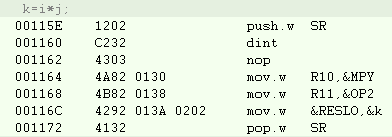
\includegraphics[width=0.7\linewidth]{img/MultF449.png}
	\captionof{figure}[Multiplikation im Assemblercodes des MSP430F499]{Multiplikation im Assemblercodes des MSP430F499 }
	\label{fig:MultF449}
\end{minipage}

Man sieht, dass die Werte von \textit{i} und \textit{j} aus den Registern R10 und R11 in die Register \textit{MPY} (Multiply unsigned/operand1) und \textit{OP2} (Second operand)\footnote{Siehe: \url{http://www.ti.com/lit/ds/symlink/msp430f449.pdf}, Seite 33} des Multiplikators geladen werden. Das Ergebnis wird anschließend aus \textit{RESLO} in \textit{k} gespeichert.

%Statusregister erwähnen?

Der MSP430F2274 muss die Aufgabe hingegen ohne Hardware-Multiplikator lösen und daher auf die aufwändige Berechnungsfunktion \textit{Mul16} zurückgreifen (siehe Abbildung \ref{fig:MultF2274} und \ref{fig:Mul16})


\vspace{1em}
\begin{minipage}{\linewidth}
	\centering
	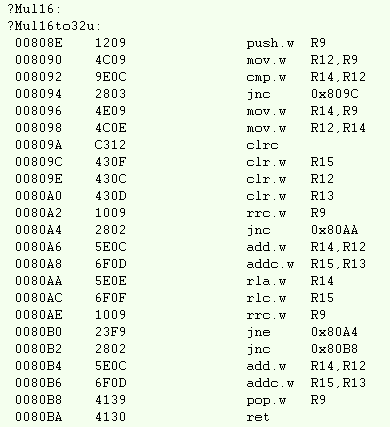
\includegraphics[width=0.7\linewidth]{img/Mul16.png}
	\captionof{figure}[Multiplikation-Funktion \textit{Mul16} im Code des MSP430F2274] {Multiplikation-Funktion \textit{Mul16} im Code des MSP430F2274}
	\label{fig:Mul16}
\end{minipage}



\pagebreak



% ----------------------------------------------------------------------------------------------------------
% Literatur
% ----------------------------------------------------------------------------------------------------------
\renewcommand\refname{Quellenverzeichnis}

%\bibliographystyle{alphadin}
%\nocite{*}
%\bibliography{bib/lit.bib}

\pagebreak

% ----------------------------------------------------------------------------------------------------------
% Anhang
% ----------------------------------------------------------------------------------------------------------
\pagenumbering{Roman}
\setcounter{page}{1}
\lhead{Anhang \thesection}

\begin{appendix}
	\section*{Anhang}
	\phantomsection
	\addcontentsline{toc}{section}{Anhang}
	\addtocontents{toc}{\vspace{-0.5em}}
	
	\section{Endfassung Lauflicht Quellcode}
	\label{sec:Lauflicht}
	Es folgt der vollständige Programm-Code:
	\vspace{1em}
	\lstinputlisting[caption=Lauflicht.c]{src/Lauflicht/blink-lauflicht_schleife.c}
	
	\pagebreak
	
	\section{Endfassung Taschenrechner Quellcode}
	\label{sec:Taschenrechner}
	Es folgt der vollständige Programm-Code:
	\vspace{1em}
	\lstinputlisting[caption=Taschenrechner.c]{src/TR/TRInterrupts.c}
	
	\pagebreak
	
	\section{Endfassung Teatimer Quellcode}
	\label{sec:Teatimer}
	Es folgt der vollständige Programm-Code:
	
	\vspace{1em}
	\lstinputlisting[caption=Teatimer.c]{src/TeaTimer/Teatimer.c}
	
	\pagebreak
	
	\section{Motorsteuerung Quellcode}
	\label{sec:Motorsteuerung}
	Es folgt der vollständige Programm-Code:
	
	\vspace{1em}
	\lstinputlisting[caption=Motorsteuerung.c]{src/Motorsteuerung/motorSteuerung.c}
	
	\pagebreak
	
	\section{Fernbedienung Quellcode}
	\label{sec:Fernbedienung}
	Es folgt der vollständige Programm-Code:
	
	\vspace{1em}
	\lstinputlisting[caption=FernbedienungTeatimer.c]{src/Fernbedienung/FernbedienungTeaTimer.c}
	
	\pagebreak
	
\end{appendix}

\pagebreak


% ----------------------------------------------------------------------------------------------------------
% Erklärung
% ----------------------------------------------------------------------------------------------------------
\thispagestyle{empty}
\begin{center}
	\vspace*{5em}
	\huge\textbf{Erklärung}\\
\end{center}
\vspace{2em}
Hiermit versicheren wir, dass wir unsere Praktikumsdokumentation selbständig verfasst und keine anderen als die angegebenen Quellen und Hilfsmittel benutzt haben.

\vspace{4em}
\begin{minipage}{\linewidth}
	\begin{tabular}{p{15em}p{15em}}
		Datum: &  .......................................................\\
		& \centering (Unterschrift)\\
	\end{tabular}
	\begin{tabular}{p{15em}p{15em}}
		Datum: &  .......................................................\\
		& \centering (Unterschrift)\\
	\end{tabular}
\end{minipage}

\end{document}
